\documentclass[11pt,a4paper]{article}
\usepackage[utf8]{inputenc}
\usepackage[margin=2.5cm]{geometry}
\usepackage{xcolor}
\usepackage{booktabs}
\usepackage{tabularx}
\usepackage{longtable}
\usepackage{array}
\usepackage{multirow}
\usepackage{graphicx}
\usepackage{subcaption}
\usepackage{tikz}
\usetikzlibrary{positioning, arrows.meta, calc, decorations.pathreplacing, fit, backgrounds, patterns}
\usepackage{hyperref}
\usepackage{fancyhdr}
\usepackage{titlesec}
\usepackage{enumitem}
\usepackage{bytefield}
\usepackage{listings}
\usepackage{tcolorbox}
\tcbuselibrary{breakable, skins}
\usepackage{amsmath}
\usepackage{etoolbox}
\usepackage{placeins}
\usepackage{float}

% === SEMANTIC COLOR PALETTE ===
\definecolor{navy}{HTML}{16213e}
\definecolor{accent}{HTML}{e94560}
\definecolor{muted}{HTML}{616161}
\definecolor{codebg}{HTML}{f4f4f4}
\definecolor{notebg}{HTML}{fff8e1}
\definecolor{noteborder}{HTML}{ffb300}
% Block-type fills (overview figures)
\definecolor{btFileHdr}{HTML}{5c6bc0}
\definecolor{btMemRegion}{HTML}{c8e6c9}
\definecolor{btMemRegionB}{HTML}{43a047}
\definecolor{btModule}{HTML}{e1bee7}
\definecolor{btModuleB}{HTML}{8e24aa}
\definecolor{btProcIdent}{HTML}{b3e5fc}
\definecolor{btProcIdentB}{HTML}{0288d1}
\definecolor{btKeyHint}{HTML}{ffe0b2}
\definecolor{btKeyHintB}{HTML}{ef6c00}
\definecolor{btEoC}{HTML}{fce4ec}
\definecolor{btEoCB}{HTML}{e94560}
\definecolor{btSysCtx}{HTML}{b2dfdb}
\definecolor{btSysCtxB}{HTML}{00897b}
\definecolor{btSysTable}{HTML}{b2dfdb}
\definecolor{btSysTableB}{HTML}{00897b}
% Common Block Header fields (payload figures)
\definecolor{hdrIdent}{HTML}{b3e5fc}
\definecolor{hdrIdentB}{HTML}{0288d1}
\definecolor{hdrUUID}{HTML}{e1bee7}
\definecolor{hdrUUIDB}{HTML}{8e24aa}
\definecolor{hdrHash}{HTML}{ffe0b2}
\definecolor{hdrHashB}{HTML}{ef6c00}
\definecolor{hdrPayload}{HTML}{fff9c4}
\definecolor{hdrPayloadB}{HTML}{f9a825}
% Payload figure fields
\definecolor{hdrBox}{HTML}{bdbdbd}
\definecolor{hdrBoxB}{HTML}{757575}
\definecolor{fldData}{HTML}{c8e6c9}
\definecolor{fldDataB}{HTML}{43a047}
\definecolor{fldUUID}{HTML}{e1bee7}
\definecolor{fldUUIDB}{HTML}{8e24aa}
\definecolor{fldCrypto}{HTML}{ffe0b2}
\definecolor{fldCryptoB}{HTML}{ef6c00}
\definecolor{fldVar}{HTML}{fff9c4}
\definecolor{fldVarB}{HTML}{f9a825}
\definecolor{fldMore}{HTML}{eeeeee}
\definecolor{fldMoreB}{HTML}{9e9e9e}
\definecolor{colReserved}{HTML}{ffcdd2}
\definecolor{colReservedB}{HTML}{c62828}
% Preamble fields (block-level, before repeated entries)
\definecolor{fldPreamble}{HTML}{b0bec5}
\definecolor{fldPreambleB}{HTML}{546e7a}
% Three-state pages
\definecolor{psCaptured}{HTML}{c8e6c9}
\definecolor{psFailed}{HTML}{ffcc80}
\definecolor{psUnmapped}{HTML}{e0e0e0}
% Encryption layout
\definecolor{encClear}{HTML}{e3f2fd}
\definecolor{encClearB}{HTML}{1565c0}
\definecolor{encCipher}{HTML}{ffccbc}
\definecolor{encCipherB}{HTML}{bf360c}
\definecolor{encTag}{HTML}{f3e5f5}
\definecolor{encTagB}{HTML}{6a1b9a}

\hypersetup{colorlinks=true, linkcolor=navy, urlcolor=accent, citecolor=navy,
    pdftitle={Memory Slice (.msl) Format Specification}}
\pagestyle{fancy}
\fancyhf{}
\fancyhead[L]{\small\color{muted}Memory Slice (.msl) Format Specification}
\fancyhead[R]{\small\color{muted}Version 1.0.0}
\fancyfoot[C]{\small\color{muted}\thepage}
\renewcommand{\headrulewidth}{0.4pt}
\renewcommand{\footrulewidth}{0pt}
\titleformat{\section}{\Large\bfseries\color{navy}}{\thesection}{1em}{}[\vspace{2pt}{\color{accent}\rule{0.25\textwidth}{1.5pt}}]
\titleformat{\subsection}{\large\bfseries\color{navy!80!black}}{\thesubsection}{1em}{}
\titleformat{\subsubsection}{\normalsize\bfseries\color{navy!60!black}}{\thesubsubsection}{1em}{}
\newtcolorbox{notebox}[1][]{colback=notebg, colframe=noteborder, fonttitle=\bfseries, #1,
    boxrule=0.5pt, arc=2pt, left=6pt, right=6pt, top=4pt, bottom=4pt, breakable}

\newcommand{\MUST}{\textbf{MUST}}
\newcommand{\MUSTNOT}{\textbf{MUST NOT}}
\newcommand{\SHALL}{\textbf{SHALL}}
\newcommand{\SHALLNOT}{\textbf{SHALL NOT}}
\newcommand{\SHOULD}{\textbf{SHOULD}}
\newcommand{\SHOULDNOT}{\textbf{SHOULD NOT}}
\newcommand{\MAY}{\textbf{MAY}}
\newcommand{\REQUIRED}{\textbf{REQUIRED}}
\newcommand{\OPTIONAL}{\textbf{OPTIONAL}}
\newcommand{\hex}[1]{\texttt{0x#1}}
\newcommand{\field}[1]{\texttt{#1}}
\newcommand{\magic}[1]{\texttt{"#1"}}
\newcommand{\padeight}{\ensuremath{\mathrm{pad8}}}
\newcommand{\blake}{BLAKE3}
\newcolumntype{M}{>{\ttfamily\small}l}
\lstset{basicstyle=\ttfamily\small, backgroundcolor=\color{codebg}, frame=single, rulecolor=\color{muted!30}, breaklines=true}

\newcommand{\blocklayout}[1]{%              
    \begin{tikzpicture}[x=0.52cm, y=0.55cm, font=\scriptsize\ttfamily,
                       every node/.style={inner sep=2pt}]
    #1
    \end{tikzpicture}}

\begin{document}
\begin{titlepage}
\vspace*{3cm}
{\color{accent}\rule{\textwidth}{3pt}}\vspace{0.5cm}
{\Huge\bfseries\color{navy} Memory Slice (.msl)\par}\vspace{0.3cm}
{\LARGE\bfseries\color{accent} Binary Format Specification\par}\vspace{0.5cm}
{\color{muted!50}\rule{\textwidth}{0.5pt}}\vspace{1cm}
{\large\color{muted}
Version: 1.0.0\\[4pt]
Status: Working Draft\\[4pt]
Editor(s): Daniel Baier\\[4pt]
This version: {\footnotesize\url{https://github.com/MemorySlice/memslice-spec/releases/tag/v1.0.0}}\\[4pt]
Latest version: {\footnotesize\url{https://github.com/MemorySlice/memslice-spec/}}
}\vspace{1.5cm}
\begin{abstract}\noindent
Memory Slice (\texttt{.msl}) is a self-describing, block-based binary format for capturing the forensic state of a single operating system process. It records both the virtual address space (with per-page acquisition status) and transient OS-queryable metadata that exists only while the process is alive. This document specifies the binary layout: file header, block architecture, integrity chain, capture-time payloads, cross-referencing, capability bitmap, raw dump import mechanism, investigation mode with system-wide context capture, and full-container AEAD encryption with post-quantum key encapsulation support.
\end{abstract}

\vfill
{\small\color{muted}
This specification accompanies the research paper \emph{Memory Slice: A Process-Centric Dump Format for Differential Memory Analysis and Volatility 3 Plugin Synthesis}.}
\end{titlepage}

\tableofcontents\newpage

%% ======================================================================
\section{Scope and Conventions}
%% ======================================================================
\subsection{Scope}
This document defines the binary wire format of Memory Slice (\texttt{.msl}) files. It does \emph{not} specify acquisition procedures or analysis algorithms.

\subsection{Normative Language}
The key words \MUST, \MUSTNOT, \REQUIRED, \SHALL, \SHALLNOT, \SHOULD, \SHOULDNOT, ``RECOMMENDED'', \MAY, and \OPTIONAL{} are per RFC~2119~\cite{rfc2119}.

\subsection{Encoding Conventions}\label{sec:encoding}
\begin{itemize}[leftmargin=1.5em, itemsep=3pt]
\item All multi-byte structural integers are \textbf{little-endian}. The file header's \field{Endianness} byte at offset~\hex{08} \MUST{} be \hex{01} in version~1.1. The field is retained for forward compatibility; future versions \MAY{} define \hex{02} (big-endian). Consumers encountering a value other than \hex{01} \MUST{} reject the file.
\item Strings are UTF-8, null-terminated, padded to \textbf{8-byte} boundaries with zero bytes. The pad function is defined as $\padeight(n) = \lceil n/8 \rceil \times 8$, where $n$ is the byte length of the UTF-8 encoded string \textbf{including} the mandatory terminating NUL (\hex{00}). All padding bytes \MUST{} be \hex{00}. Textual string fields \MUSTNOT{} contain \hex{00} bytes before the terminating NUL.
\item Where a string field is accompanied by an explicit length field (e.g., \field{PathLen}, \field{ExePathLen}), the \textbf{length field is authoritative}: it specifies the byte count including the terminating NUL. The on-disk storage occupies $\padeight(\text{Len})$ bytes. Consumers \MUST{} use the length field to determine string extent and \MUSTNOT{} scan beyond \field{Len} bytes. The NUL byte at position $\text{Len}-1$ serves as a consistency check.
\item Producers \MUST{} emit well-formed UTF-8 per RFC~3629~\cite{rfc3629}. Consumers encountering invalid UTF-8 sequences \SHOULD{} preserve the raw bytes and \MAY{} flag the field as malformed, but \MUSTNOT{} reject the entire block. This ensures that forensic evidence is never silently discarded due to encoding errors in captured metadata.
\item Variable-length fields (\field{PageStateMap}, \field{NativeBlob}) are padded to 8-byte boundaries.
\item UUIDs \MUST{} be version~4 (random) per RFC~9562~\cite{rfc9562}, stored as 16 raw bytes in RFC~9562 binary layout. See Section~\ref{sec:uuids}.
\item Integrity hashes use the algorithm selected by \field{HashAlgo} (Section~\ref{sec:hashchain}); all registered algorithms produce 32-byte output. The default is BLAKE3~\cite{blake3}.
\item Timestamps: unsigned 64-bit nanoseconds since Unix epoch (1970-01-01T00:00:00Z).
\item All \field{Reserved} fields \MUST{} be zero (producers) and \MUST{} be ignored (consumers).
\end{itemize}

\subsection{Byte Order Domains}\label{sec:byteorder}
Three byte-order regimes coexist within an MSL file. Implementers \MUST{} observe the boundaries precisely:
\begin{enumerate}[leftmargin=1.8em, itemsep=2pt]
\item \textbf{Structural integers.} All multi-byte integers in the file header, block headers, and payload fixed fields are little-endian (controlled by \field{Endianness}=\hex{01}).
\item \textbf{UUIDs.} All UUID fields are stored in RFC~9562 binary layout (big-endian mixed-endian per the RFC) and are \emph{never} subject to byte-swapping, regardless of the file's \field{Endianness} setting.
\item \textbf{Captured memory content.} Bytes within \field{PageData} are stored verbatim in the target architecture's native byte order; the format does not reorder them.
\end{enumerate}

\subsection{UUID Requirements}\label{sec:uuids}
All UUID fields (\field{DumpUUID}, \field{BlockUUID}, \field{ParentUUID}, payload UUIDs) \MUST{} be version~4 (random) per RFC~9562. The 4-bit version field (bits 48--51) \MUST{} be \texttt{0100}; the 2-bit variant (bits 64--65) \MUST{} be \texttt{10}. UUIDs are stored as 16-byte sequences in RFC~9562 binary layout and are never subject to byte-swapping.

\begin{notebox}[title={Implementation guidance: UUID generation}]
A thread-local fast PRNG such as \texttt{xoshiro256++} or \texttt{PCG64}, seeded once from OS entropy, provides sufficient uniqueness ($\sim\!2^{-61}$ collision probability per pair) while avoiding CSRNG overhead per block. Note that this is a \emph{performance optimization}, not a conformance requirement; implementations \MAY{} use a CSRNG if preferred.
\end{notebox}

\subsection{Terminology}
\begin{description}[style=nextline, leftmargin=2em, itemsep=4pt]
\item[Producer] Software that creates or appends blocks.
\item[Consumer] Software that reads an MSL file.
\item[Acquirer] A producer capturing live process state (types \hex{0000}--\hex{0FFF}).
\item[Importer] A producer converting a raw dump into MSL (Section~\ref{sec:import}).
\item[Block] Fixed header + variable payload.
\item[Payload] Block-type-specific data after the header.
\item[Preamble] Block-level fields at the start of a payload that precede repeated entry structures (e.g., \field{EntryCount}).
\item[Investigation Mode] Acquisition for forensic investigations with system-wide context (Section~\ref{sec:investigation}).
\item[Analysis Mode] Default mode for research and tool development. No system-wide context required.
\end{description}

\vspace{1em}\noindent\rule{\textwidth}{0.3pt}\vspace{0.5em}
\noindent\textit{The following sections define the format itself, starting with the high-level file structure.}

\newpage
%% ======================================================================
\section{Format Overview}\label{sec:overview}
%% ======================================================================
An MSL file is a linear byte stream: a \textbf{file header} followed by \textbf{typed, length-prefixed blocks}. No inter-block gaps. \field{HeaderSize} tells the consumer where blocks begin. Figure~\ref{fig:format-overview} shows the high-level structure.

\begin{figure}[H]
\centering
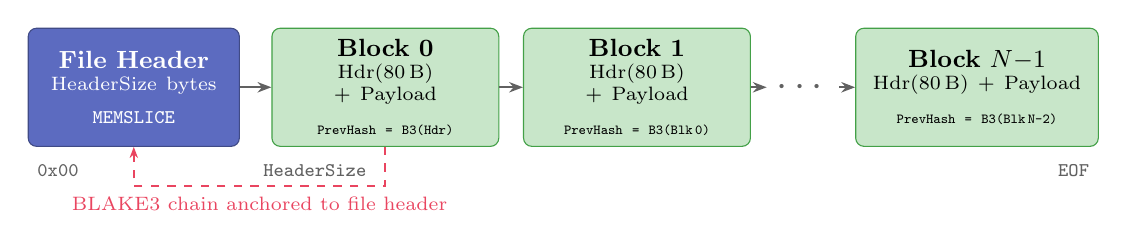
\begin{tikzpicture}[
    block/.style={draw, rounded corners=3pt, minimum height=1.5cm, text width=#1, align=center, inner sep=4pt},
    arr/.style={-{Stealth[length=5pt]}, thick, color=muted},
    lbl/.style={font=\scriptsize\ttfamily, color=muted},
]
\node[block=2.4cm, fill=btFileHdr, draw=btFileHdr!70!black, text=white] (hdr) {\small\textbf{File Header}\\\scriptsize HeaderSize bytes\\\scriptsize\texttt{MEMSLICE}};
\node[block=2.6cm, fill=btMemRegion, draw=btMemRegionB, right=0.4cm of hdr] (b0) {\small\textbf{Block 0}\\\scriptsize Hdr(80\,B) + Payload\\\tiny\texttt{PrevHash = B3(Hdr)}};
\node[block=2.6cm, fill=btMemRegion, draw=btMemRegionB, right=0.3cm of b0] (b1) {\small\textbf{Block 1}\\\scriptsize Hdr(80\,B) + Payload\\\tiny\texttt{PrevHash = B3(Blk\,0)}};
\node[right=0.2cm of b1, font=\Large\bfseries, color=muted] (dots) {$\cdots$};
\node[block=2.8cm, fill=btMemRegion, draw=btMemRegionB, right=0.2cm of dots] (bn) {\small\textbf{Block $N{-}1$}\\\scriptsize Hdr(80\,B) + Payload\\\tiny\texttt{PrevHash = B3(Blk\,N{-}2)}};
\draw[arr] (hdr)--(b0); \draw[arr] (b0)--(b1); \draw[arr] (b1)--(dots); \draw[arr] (dots)--(bn);
\node[lbl, below=3pt of hdr.south west, anchor=north west] {0x00};
\node[lbl, below=3pt of hdr.south east, anchor=north west] {\, HeaderSize};
\node[lbl, below=3pt of bn.south east, anchor=north east] {EOF};
\draw[thick, dashed, color=accent, -{Stealth[length=4pt]}] (b0.south)--++(0,-0.5)-| node[pos=0.25, below, font=\scriptsize\color{accent}] {\blake{} chain anchored to file header} (hdr.south);
\end{tikzpicture}
\caption{MSL file structure: file header followed by \blake{}-chained blocks.}
\label{fig:format-overview}
\end{figure}

Block~0's \field{PrevHash} = $\blake(\text{File Header})$. Each subsequent block hashes its predecessor. Consumers detect end-of-file when fewer than 80 bytes remain or the next 4 bytes do not match the block magic (\hex{4D534C43}). If \field{BlockCount} in the file header is non-zero, consumers \SHOULD{} additionally verify that the parsed block count matches the declared value.

\subsection{Acquisition Modes}\label{sec:modes}
The file header's \field{Flags} field (offset~\hex{0C}) determines the acquisition mode and whether encryption is active:

\begin{description}[style=nextline, leftmargin=2em, itemsep=4pt]
\item[\textbf{Analysis Mode} (\field{Investigation}=0)] The default. For research and developing new forensic approaches. Header is 64~bytes. No system-wide context required. Figure~\ref{fig:acq-sequence}.
\item[\textbf{Investigation Mode} (\field{Investigation}=1)] For forensic investigations. Block~2 \MUST{} be a System Context block (\hex{0050}). Section~\ref{sec:investigation}. Figure~\ref{fig:inv-combined}.
\end{description}

\noindent Either mode \MAY{} set the \field{Encrypted} flag (bit~2), activating full-container Authenticated Encryption with Associated Data (AEAD) as defined in Section~\ref{sec:encryption}. When set, \field{HeaderSize} is~128 and the entire block stream is encrypted. Table~\ref{tab:mode-summary} summarizes the combinations.

\begin{table}[H]\centering\caption{Acquisition mode and encryption flag combinations.}\label{tab:mode-summary}\small
\begin{tabular}{l l l l}\toprule\textbf{Investigation} & \textbf{Encrypted} & \textbf{HeaderSize} & \textbf{Block~2}\\\midrule
0 & 0 & 64 & Memory Region or other capture-time block \\
0 & 1 & 128 & Memory Region or other (encrypted) \\
1 & 0 & 64 & System Context (\hex{0050}, \REQUIRED) \\
1 & 1 & 128 & System Context (\hex{0050}, \REQUIRED, encrypted) \\
\bottomrule\end{tabular}\end{table}

\begin{figure}[H]
\centering
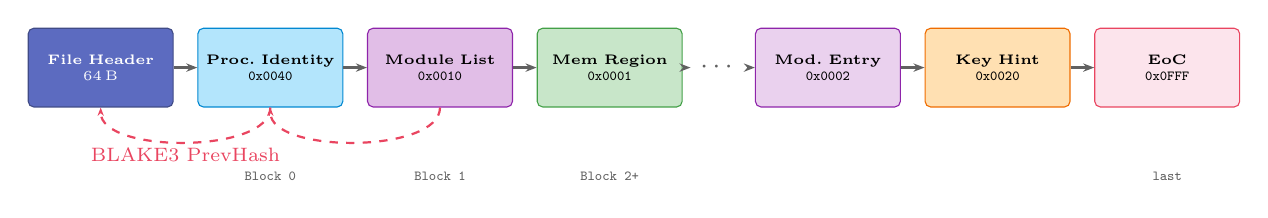
\begin{tikzpicture}[blk/.style={draw, rounded corners=2pt, minimum height=1.0cm, text width=1.7cm, align=center, inner sep=2pt, font=\tiny},lbl/.style={font=\tiny\ttfamily, color=muted},arr/.style={-{Stealth[length=4pt]}, thick, color=muted}]
\node[blk, fill=btFileHdr, draw=btFileHdr!70!black, text=white] (hdr) at (0,0) {\textbf{File Header}\\64\,B};
\node[blk, fill=btProcIdent, draw=btProcIdentB, right=0.3cm of hdr] (b0) {\textbf{Proc.\ Identity}\\\hex{0040}};
\node[blk, fill=btModule, draw=btModuleB, right=0.3cm of b0] (b1) {\textbf{Module List}\\\hex{0010}};
\node[blk, fill=btMemRegion, draw=btMemRegionB, right=0.3cm of b1] (b2) {\textbf{Mem Region}\\\hex{0001}};
\node[right=0.1cm of b2, font=\normalsize\bfseries, color=muted] (dots) {$\cdots$};
\node[blk, fill=btModule!70, draw=btModuleB, right=0.1cm of dots] (bm) {\textbf{Mod.\ Entry}\\\hex{0002}};
\node[blk, fill=btKeyHint, draw=btKeyHintB, right=0.3cm of bm] (bk) {\textbf{Key Hint}\\\hex{0020}};
\node[blk, fill=btEoC, draw=btEoCB, right=0.3cm of bk] (eoc) {\textbf{EoC}\\\hex{0FFF}};
\draw[arr] (hdr)--(b0); \draw[arr] (b0)--(b1); \draw[arr] (b1)--(b2); \draw[arr] (b2)--(dots); \draw[arr] (dots)--(bm); \draw[arr] (bm)--(bk); \draw[arr] (bk)--(eoc);
\node[lbl, below=0.7cm of b0.south] {Block 0}; \node[lbl, below=0.7cm of b1.south] {Block 1}; \node[lbl, below=0.7cm of b2.south] {Block 2+}; \node[lbl, below=0.7cm of eoc.south] {last};
\draw[-{Stealth[length=3pt]}, thick, dashed, color=accent] (b0.south) to[out=-90, in=-90, looseness=0.7] (hdr.south);
\node[font=\scriptsize\color{accent}] at ($(hdr.south)!0.5!(b0.south)+(0,-0.6)$) {\blake{} PrevHash};
\draw[-{Stealth[length=3pt]}, thick, dashed, color=accent] (b1.south) to[out=-90, in=-90, looseness=0.7] (b0.south);
\end{tikzpicture}
\caption{Analysis mode (\field{Investigation}=0, \field{Encrypted}=0).}
\label{fig:acq-sequence}
\end{figure}

\begin{figure}[H]
\centering
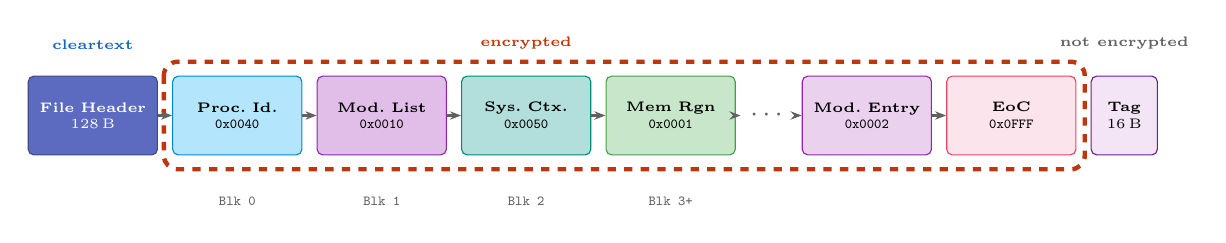
\begin{tikzpicture}[blk/.style={draw, rounded corners=2pt, minimum height=1.0cm, text width=1.5cm, align=center, inner sep=2pt, font=\tiny},lbl/.style={font=\tiny\ttfamily, color=muted},arr/.style={-{Stealth[length=4pt]}, thick, color=muted},zonelbl/.style={font=\tiny\bfseries}]
\node[blk, fill=btFileHdr, draw=btFileHdr!70!black, text=white] (hdr) at (0,0) {\textbf{File Header}\\128\,B};
\node[blk, fill=btProcIdent, draw=btProcIdentB, right=0.18cm of hdr] (b0) {\textbf{Proc.\ Id.}\\\hex{0040}};
\node[blk, fill=btModule, draw=btModuleB, right=0.18cm of b0] (b1) {\textbf{Mod.\ List}\\\hex{0010}};
\node[blk, fill=btSysCtx, draw=btSysCtxB, right=0.18cm of b1] (b2) {\textbf{Sys.\ Ctx.}\\\hex{0050}};
\node[blk, fill=btMemRegion, draw=btMemRegionB, right=0.18cm of b2] (b3) {\textbf{Mem Rgn}\\\hex{0001}};
\node[right=0.06cm of b3, font=\normalsize\bfseries, color=muted] (dots) {$\cdots$};
\node[blk, fill=btModule!70, draw=btModuleB, right=0.06cm of dots] (bm) {\textbf{Mod.\ Entry}\\\hex{0002}};
\node[blk, fill=btEoC, draw=btEoCB, right=0.18cm of bm] (eoc) {\textbf{EoC}\\\hex{0FFF}};
\node[blk, text width=0.7cm, fill=encTag, draw=encTagB, right=0.18cm of eoc] (tag) {\textbf{Tag}\\16\,B};
\draw[arr] (hdr)--(b0); \draw[arr] (b0)--(b1); \draw[arr] (b1)--(b2); \draw[arr] (b2)--(b3); \draw[arr] (b3)--(dots); \draw[arr] (dots)--(bm); \draw[arr] (bm)--(eoc);
\node[lbl, below=0.4cm of b0.south] {Blk 0}; \node[lbl, below=0.4cm of b1.south] {Blk 1}; \node[lbl, below=0.4cm of b2.south] {Blk 2}; \node[lbl, below=0.4cm of b3.south] {Blk 3+};
\node[zonelbl, color=encClearB, above=6pt of hdr.north] {cleartext};
\begin{scope}[on background layer]
\draw[ultra thick, color=encCipherB, dashed, rounded corners=5pt] ([xshift=-3pt, yshift=5pt]b0.north west) rectangle ([xshift=3pt, yshift=-5pt]eoc.south east);
\end{scope}
\node[zonelbl, color=encCipherB, above=6pt of b2.north] {encrypted};
\node[zonelbl, color=muted, above=6pt of tag.north] {not encrypted};
\end{tikzpicture}
\caption{Investigation mode with encryption (\field{Investigation}=1, \field{Encrypted}=1). The 16-byte authentication tag is an \emph{output} of the AEAD, not itself encrypted.}
\label{fig:inv-combined}
\end{figure}

\subsection{Design Principles}
\begin{enumerate}[leftmargin=1.8em, itemsep=2pt]
\item \textbf{Integrity Verification.} Append-only policy with \blake{} hash chain.
\item \textbf{Epistemic Honesty.} Three-state pages: Captured vs.\ Failed vs.\ Unmapped.
\item \textbf{Self-Describing.} Version, header size, OS, arch, PID, capabilities.
\item \textbf{Dual-Layer OS Abstraction.} Normalized fields + OS-native opaque blob.
\item \textbf{Dual Acquisition Modes.} Analysis mode for research; Investigation mode for forensic investigations.
\item \textbf{Confidentiality.} Full-container AEAD encryption with post-quantum key encapsulation.
\end{enumerate}

Capture-time blocks are optimized for streaming, append-only acquisition. The Structural namespace (\hex{1000}--\hex{1FFF}) is reserved for analysis tools to add post-acquisition indexes---including seek tables and virtual address maps---that enable efficient random access without modifying the capture-time block stream.

\subsection{Scope of the Integrity Guarantee}\label{sec:integrityscope}
The hash chain provides \emph{tamper detection}, not \emph{tamper resistance}. It protects against \textbf{accidental corruption} and detects \textbf{naive modification}, including block reordering, insertion, and deletion---threats that a per-block checksum alone cannot detect, since the chain cryptographically binds each block to its predecessor and ultimately to the file header. For tamper evidence admissible in legal contexts, producers \SHOULD{} complement the hash chain with external mechanisms (digital signature over \field{FileHash}, RFC~3161 timestamp, write-once media). When encryption is active, the AEAD tag provides stronger integrity. The hash chain alone \MUSTNOT{} be represented as providing forensic-grade tamper evidence.

\begin{table}[H]\centering\caption{Integrity mechanisms: guarantees and limitations.}\label{tab:threatmodel}\small
\begin{tabular}{l p{3.5cm} p{4cm} l}\toprule\textbf{Mechanism}&\textbf{Protects Against}&\textbf{Limitations}&\textbf{Key?}\\\midrule
\blake{} chain & Accidental corruption, naive modification & Attacker can recompute chain after modification & No \\
EoC \field{FileHash} & Truncation, missing blocks & Recomputable by attacker; only verifiable after decryption if encrypted & No \\
AEAD tag & Any tampering of encrypted block stream & Header remains cleartext (metadata leakage); requires key compromise to forge & Yes \\
External hash & Complete file substitution, transport corruption & Only as trustworthy as the storage of the hash itself & No \\
\bottomrule\end{tabular}\end{table}

%% ======================================================================
\newpage
\section{File Header}\label{sec:fileheader}
%% ======================================================================

\subsection{Base Header (64 bytes)}\label{sec:basehdr}

\begin{table}[H]\centering\caption{File header (64 bytes minimum; 128 when \field{Encrypted}).}\label{tab:fileheader}\small
\begin{tabular}{M M l l p{4.5cm}}\toprule\textbf{Offset}&\textbf{Size}&\textbf{Field}&\textbf{Abbr}&\textbf{Description}\\\midrule
0x00 & 8  & \field{Magic}      & --- & \hex{4D454D534C494345} (\magic{MEMSLICE}). \\
0x08 & 1  & \field{Endianness} & E & v1.1: \MUST{} be \hex{01} (LE). \hex{02} (BE) reserved for future versions. Other values \MUST{} cause rejection. \\
0x09 & 1  & \field{HeaderSize} & HS & \hex{40}~(64) for unencrypted; \hex{80}~(128) when \field{Encrypted}. First block (or Key Encapsulation Mechanism ciphertext) starts here. \\
0x0A & 2  & \field{Version}    & Ver & \texttt{uint16}. Major in high byte, minor in low: v1.1~=~\hex{0101}. \\
0x0C & 4  & \field{Flags}      & --- & See Table~\ref{tab:hdrflags}. \\
0x10 & 8  & \field{CapBitmap}  & CapBm & Capability bitmap (Section~\ref{sec:capbitmap}). \\
0x18 & 16 & \field{DumpUUID}   & --- & UUIDv4 uniquely identifying this dump. \\
0x28 & 8  & \field{Timestamp}  & Ts & Acquisition start (UTC, ns since epoch). \\
0x30 & 2  & \field{OSType}     & OS & Target OS (Table~\ref{tab:platformcodes}a). \\
0x32 & 2  & \field{ArchType}   & Ar & Target CPU (Table~\ref{tab:platformcodes}b). \\
0x34 & 4  & \field{PID}        & --- & Process ID at acquisition. \\
0x38 & 1  & \field{ClockSource} & CS & \hex{00}=Unknown, \hex{01}=\texttt{CLOCK\_REALTIME}, \hex{02}=\texttt{CLOCK\_MONOTONIC\_RAW}, \hex{03}=\texttt{QPC}, \hex{04}=\texttt{mach\_absolute\_time}. \hex{FF}=Other. \\
0x39 & 4  & \field{BlockCount} & BCt & Total number of blocks (incl.\ EoC). \hex{00000000}~=~unknown (streaming). Consumers \SHOULD{} verify if non-zero. \\
0x3D & 1  & \field{HashAlgo}   & HA & Integrity hash algorithm selector (Table~\ref{tab:hashalgos}). \hex{00}=BLAKE3 (default). \\
0x3E & 2  & \field{Reserved}   & Rsv & \MUST{} be zero. \\
\bottomrule\end{tabular}\end{table}

\noindent\textbf{Size:} $8{+}1{+}1{+}2{+}4{+}8{+}16{+}8{+}2{+}2{+}4{+}1{+}4{+}1{+}2=64$.

\begin{notebox}[title={BlockCount semantics}]
A producer that writes blocks in streaming fashion (i.e., the total count is unknown at file creation time) \MUST{} write \hex{00000000}. Such a producer \MAY{} seek back after writing the EoC block and patch \field{BlockCount} to the actual value. When \field{BlockCount} is non-zero and the number of successfully parsed blocks differs, the file \SHOULD{} be considered truncated or corrupt.
\end{notebox}

\begin{table}[H]\centering\caption{File header flags (\field{Flags}, 32~bits at offset~\hex{0C}).}\label{tab:hdrflags}\small
\begin{tabular}{l l p{8.5cm}}\toprule\textbf{Bit}&\textbf{Name}&\textbf{Description}\\\midrule
0 & \field{Imported} & File created by importing a raw dump (Section~\ref{sec:import}). \\
1 & \field{Investigation} & Forensic investigation. System Context block (\hex{0050}) \MUST{} be Block~2 (Section~\ref{sec:investigation}). \\
2 & \field{Encrypted} & Full-container AEAD encryption. \field{HeaderSize} \MUST{} be~128 (Section~\ref{sec:encryption}). \\
3 & \field{Redacted} & One or more fields have been intentionally stripped or pseudonymized (Section~\ref{sec:redaction}). \\
4--31 & Reserved & Zero. \\
\bottomrule\end{tabular}\end{table}

\noindent When \field{Investigation} is set and \field{Encrypted} is not, confidentiality \SHOULD{} be ensured by external means (e.g., full-disk encryption, physically secured storage). Unencrypted Investigation mode is appropriate when the goal is rapid triage or when organizational policy provides confidentiality at the storage layer.

\subsection{Encryption Extension Header (\hex{40}--\hex{7F})}\label{sec:enchdr}
When \field{Encrypted} is set, \field{HeaderSize} \MUST{} be~128. Bytes \hex{00}--\hex{3F} retain the base layout; bytes \hex{40}--\hex{7F} carry encryption parameters (Table~\ref{tab:enctable}).

\begin{table}[H]\centering\caption{Encryption extension header (64 bytes at \hex{40}--\hex{7F}).}\label{tab:enctable}\small
\begin{tabular}{M M l l p{4cm}}\toprule\textbf{Off}&\textbf{Size}&\textbf{Field}&\textbf{Abbr}&\textbf{Description}\\\midrule
0x40 & 1  & \field{EncAlgo}  & EA & AEAD cipher suite (Table~\ref{tab:ciphers}). \\
0x41 & 1  & \field{KDFType}  & KD & \hex{00}=None, \hex{01}=Argon2id. \\
0x42 & 1  & \field{KeyEncap} & KE & Key encapsulation (Table~\ref{tab:kem}). \hex{00}=None. \\
0x43 & 1  & \field{Reserved} & R & Zero. \\
0x44 & 4  & \field{KDFTime}  & KTm & Argon2id time cost. 0 if N/A. \\
0x48 & 4  & \field{KDFMemory}& KMm & Argon2id memory (KiB). 0 if N/A. \\
0x4C & 1  & \field{KDFLanes} & L & Argon2id parallelism. 0 if N/A. \\
0x4D & 1  & \field{Reserved2}& R & Zero. \\
0x4E & 2  & \field{KEMCtLen} & KCL & KEM ciphertext length. 0 when \field{KeyEncap}=\hex{00}. \\
0x50 & 24 & \field{Nonce}    & --- & AEAD nonce. AES-256-GCM: 12B used, rest zero. XChaCha20-Poly1305: all 24B. \\
0x68 & 16 & \field{KDFSalt}  & --- & KDF salt. Zeros if N/A. \\
0x78 & 8  & \field{Reserved3}& Rsv & Zero. \\
\bottomrule\end{tabular}\end{table}

\noindent\textbf{Size:} $1{+}1{+}1{+}1{+}4{+}4{+}1{+}1{+}2{+}24{+}16{+}8 = 64$. Total header: $64{+}64=128$.

\noindent The extension carries all parameters needed to decrypt the block stream: the cipher suite, KDF configuration (for passphrase-derived keys), Key Encapsulation Mechanism (KEM) ciphertext length, the AEAD nonce, and the KDF salt. Figure~\ref{fig:ext-header} shows the combined 128-byte header layout with base and extension regions.

\begin{figure}[H]
\centering
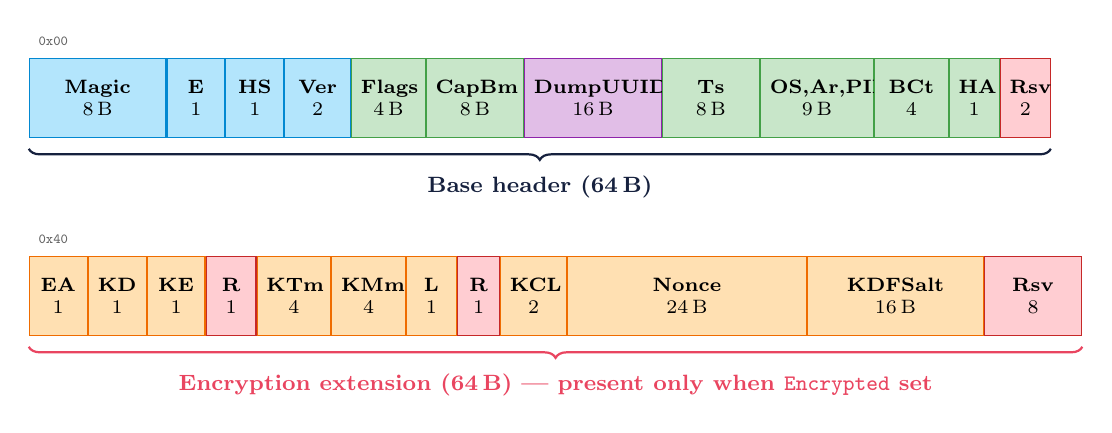
\begin{tikzpicture}[fld/.style={draw, minimum height=1.0cm, align=center, font=\scriptsize},lbl/.style={font=\tiny\ttfamily, color=muted}]
\node[fld, text width=1.5cm, fill=hdrIdent, draw=hdrIdentB] (magic) at (0,0) {\textbf{Magic}\\8\,B};
\node[fld, text width=0.5cm, fill=hdrIdent, draw=hdrIdentB, right=0pt of magic] (end) {\textbf{E}\\1};
\node[fld, text width=0.5cm, fill=hdrIdent, draw=hdrIdentB, right=0pt of end] (hs) {\textbf{HS}\\1};
\node[fld, text width=0.6cm, fill=hdrIdent, draw=hdrIdentB, right=0pt of hs] (ver) {\textbf{Ver}\\2};
\node[fld, text width=0.7cm, fill=fldData, draw=fldDataB, right=0pt of ver] (flg) {\textbf{Flags}\\4\,B};
\node[fld, text width=1.0cm, fill=fldData, draw=fldDataB, right=0pt of flg] (cap) {\textbf{CapBm}\\8\,B};
\node[fld, text width=1.5cm, fill=hdrUUID, draw=hdrUUIDB, right=0pt of cap] (duuid) {\textbf{DumpUUID}\\16\,B};
\node[fld, text width=1.0cm, fill=fldData, draw=fldDataB, right=0pt of duuid] (ts) {\textbf{Ts}\\8\,B};
\node[fld, text width=1.2cm, fill=fldData, draw=fldDataB, right=0pt of ts] (rest) {\textbf{OS,Ar,PID,CS}\\9\,B};
\node[fld, text width=0.7cm, fill=fldData, draw=fldDataB, right=0pt of rest] (bct) {\textbf{BCt}\\4};
\node[fld, text width=0.4cm, fill=fldData, draw=fldDataB, right=0pt of bct] (ha) {\textbf{HA}\\1};
\node[fld, text width=0.4cm, fill=colReserved, draw=colReservedB, right=0pt of ha] (r1) {\textbf{Rsv}\\2};
\draw[decorate, decoration={brace, amplitude=4pt, mirror, raise=4pt}, thick, color=navy] (magic.south west)--(r1.south east) node[midway, below=10pt, font=\footnotesize\bfseries\color{navy}] {Base header (64\,B)};
\node[fld, text width=0.5cm, fill=fldCrypto, draw=fldCryptoB, anchor=north west] (ea) at ([yshift=-1.5cm]magic.south west) {\textbf{EA}\\1};
\node[fld, text width=0.5cm, fill=fldCrypto, draw=fldCryptoB, right=0pt of ea] (kdf) {\textbf{KD}\\1};
\node[fld, text width=0.5cm, fill=fldCrypto, draw=fldCryptoB, right=0pt of kdf] (ke) {\textbf{KE}\\1};
\node[fld, text width=0.4cm, fill=colReserved, draw=colReservedB, right=0pt of ke] (r2) {\textbf{R}\\1};
\node[fld, text width=0.7cm, fill=fldCrypto, draw=fldCryptoB, right=0pt of r2] (kt) {\textbf{KTm}\\4};
\node[fld, text width=0.7cm, fill=fldCrypto, draw=fldCryptoB, right=0pt of kt] (km) {\textbf{KMm}\\4};
\node[fld, text width=0.4cm, fill=fldCrypto, draw=fldCryptoB, right=0pt of km] (kl) {\textbf{L}\\1};
\node[fld, text width=0.3cm, fill=colReserved, draw=colReservedB, right=0pt of kl] (r3) {\textbf{R}\\1};
\node[fld, text width=0.6cm, fill=fldCrypto, draw=fldCryptoB, right=0pt of r3] (kcl) {\textbf{KCL}\\2};
\node[fld, text width=2.8cm, fill=fldCrypto, draw=fldCryptoB, right=0pt of kcl] (nonce) {\textbf{Nonce}\\24\,B};
\node[fld, text width=2.0cm, fill=fldCrypto, draw=fldCryptoB, right=0pt of nonce] (salt) {\textbf{KDFSalt}\\16\,B};
\node[fld, text width=1.0cm, fill=colReserved, draw=colReservedB, right=0pt of salt] (r4) {\textbf{Rsv}\\8};
\draw[decorate, decoration={brace, amplitude=4pt, mirror, raise=4pt}, thick, color=accent] (ea.south west)--(r4.south east) node[midway, below=10pt, font=\footnotesize\bfseries\color{accent}] {Encryption extension (64\,B) --- present only when \field{Encrypted} set};
\node[lbl, above=1pt of magic.north west, anchor=south west] {\hex{00}};
\node[lbl, above=1pt of ea.north west, anchor=south west] {\hex{40}};
\end{tikzpicture}
\caption{Extended file header (128~bytes). Abbreviations per Tables~\ref{tab:fileheader} and~\ref{tab:enctable}.}
\label{fig:ext-header}
\end{figure}

\subsection{Byte Order}
All multi-byte structural integers are little-endian (\field{Endianness}=\hex{01}). Memory content within \field{PageData} is stored in the target architecture's native order. See Section~\ref{sec:byteorder} for the complete byte-order domain summary.

\subsection{Version Compatibility}
Unknown major version: \SHOULD{} reject. Unknown minor of known major: \MAY{} parse. Always use \field{HeaderSize} to locate Block~0.

\begin{table}[H]\centering\caption{Target platform codes: (a) OS and (b) CPU.}\label{tab:platformcodes}\small
\begin{minipage}[t]{0.47\textwidth}\centering
\subcaption*{\textbf{(a) OS type codes} (\field{OSType})}
\begin{tabular}{M l}\toprule\textbf{Code}&\textbf{OS}\\\midrule
0x0000 & Windows \\ 0x0001 & Linux \\ 0x0002 & macOS \\ 0x0003 & Android \\
0x0004 & iOS/iPadOS \\ 0x0005 & FreeBSD \\ 0x0006 & NetBSD \\ 0x0007 & OpenBSD \\
0x0008 & QNX \\ 0x0009 & Fuchsia \\
0x000A--0x00FF & \textit{Reserved} \\ 0x0100--0xFFFE & \textit{Vendor} \\ 0xFFFF & Unknown \\\bottomrule
\end{tabular}\end{minipage}%
\hfill
\begin{minipage}[t]{0.47\textwidth}\centering
\subcaption*{\textbf{(b) Architecture codes} (\field{ArchType})}
\begin{tabular}{M l}\toprule\textbf{Code}&\textbf{Architecture}\\\midrule
0x0000 & x86 (IA-32) \\ 0x0001 & x86\_64 (AMD64) \\ 0x0002 & ARM64 (AArch64) \\
0x0003 & ARM32 \\ 0x0004 & MIPS32 \\ 0x0005 & MIPS64 \\ 0x0006 & RISC-V RV32 \\
0x0007 & RISC-V RV64 \\ 0x0008 & PPC32 \\ 0x0009 & PPC64 \\ 0x000A & s390x \\
0x000B & LoongArch64 \\
0x000C--0x00FF & \textit{Reserved} \\ 0x0100--0xFFFE & \textit{Vendor} \\ 0xFFFF & Unknown \\\bottomrule
\end{tabular}\end{minipage}
\end{table}

%% ======================================================================
\newpage
\section{Block Architecture}\label{sec:blocks}
%% ======================================================================
Every block consists of a \textbf{fixed 80-byte Common Block Header} followed by a \textbf{variable-length payload}. \field{BlockLength} specifies the total \textbf{on-disk} size of the block (header + payload, in compressed form if applicable). Consumers \MUST{} verify $\field{BlockLength} \geq 80$ and \MUST{} reject blocks that violate this constraint. Unknown types are skipped via \field{BlockLength}.

\subsection{Common Block Header (80 bytes)}\label{sec:blockheader}
Every block begins with the same 80-byte header, which provides type identification, length framing, UUID-based identity and parentage, and the \blake{} integrity chain anchor. The fixed header size ensures that consumers can always parse block boundaries without understanding payload formats. Table~\ref{tab:blockheader} defines the fields; Figure~\ref{fig:block-header} shows the layout.

\begin{table}[H]\centering\caption{Block header (80 bytes). All fields $\geq$\,8\,B are 8-byte aligned.}\label{tab:blockheader}\small
\begin{tabular}{M M l l p{4.5cm}}\toprule\textbf{Off}&\textbf{Size}&\textbf{Field}&\textbf{Abbr}&\textbf{Description}\\\midrule
0x00 & 4  & \field{Magic} & --- & \hex{4D534C43} (\magic{MSLC}). \\
0x04 & 2  & \field{BlockType} & Type & Payload selector (Section~\ref{sec:typeregs}). \\
0x06 & 2  & \field{Flags} & --- & Per-block flags (Table~\ref{tab:blockflags}). \\
0x08 & 4  & \field{BlockLength} & Len & Total on-disk size (hdr+payload). $\geq 80$. \\
0x0C & 2  & \field{PayloadVersion} & PVer & Default: \hex{0001}. \\
0x0E & 2  & \field{Reserved} & R & Zero. \\
0x10 & 16 & \field{BlockUUID} & BlkUUID & UUIDv4. 8-byte aligned. \\
0x20 & 16 & \field{ParentUUID} & ParUUID & Parent or zeros. 8-byte aligned. \\
0x30 & 32 & \field{PrevHash} & --- & \blake{} of preceding element. Zeros when encrypted. 8-byte aligned. \\
0x50 & var& \field{Payload} & --- & $\field{BlockLength}-80$ bytes. \\
\bottomrule\end{tabular}\end{table}

\begin{figure}[H]
\centering
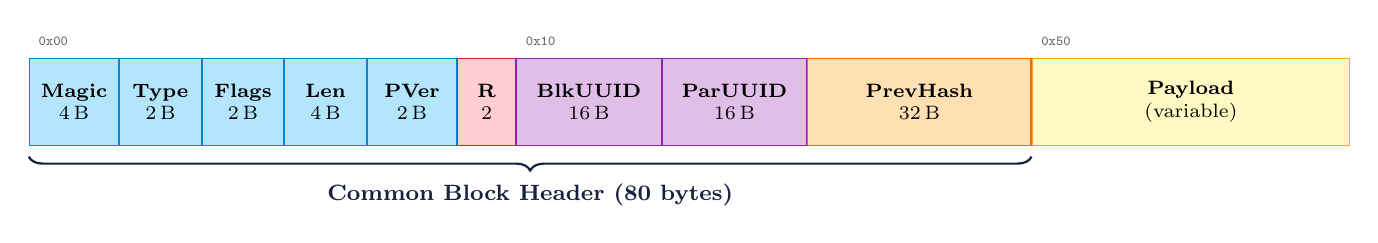
\begin{tikzpicture}[fld/.style={draw, minimum height=1.1cm, align=center, font=\scriptsize},lbl/.style={font=\tiny\ttfamily, color=muted}]
\node[fld, text width=0.9cm, fill=hdrIdent, draw=hdrIdentB] (magic) at (0,0) {\textbf{Magic}\\4\,B};
\node[fld, text width=0.8cm, fill=hdrIdent, draw=hdrIdentB, right=0pt of magic] (type) {\textbf{Type}\\2\,B};
\node[fld, text width=0.8cm, fill=hdrIdent, draw=hdrIdentB, right=0pt of type] (flags) {\textbf{Flags}\\2\,B};
\node[fld, text width=0.8cm, fill=hdrIdent, draw=hdrIdentB, right=0pt of flags] (len) {\textbf{Len}\\4\,B};
\node[fld, text width=0.9cm, fill=hdrIdent, draw=hdrIdentB, right=0pt of len] (pver) {\textbf{PVer}\\2\,B};
\node[fld, text width=0.5cm, fill=colReserved, draw=colReservedB, right=0pt of pver] (resv) {\textbf{R}\\2};
\node[fld, text width=1.6cm, fill=hdrUUID, draw=hdrUUIDB, right=0pt of resv] (buuid) {\textbf{BlkUUID}\\16\,B};
\node[fld, text width=1.6cm, fill=hdrUUID, draw=hdrUUIDB, right=0pt of buuid] (puuid) {\textbf{ParUUID}\\16\,B};
\node[fld, text width=2.6cm, fill=hdrHash, draw=hdrHashB, right=0pt of puuid] (phash) {\textbf{PrevHash}\\32\,B};
\node[fld, text width=3.8cm, fill=hdrPayload, draw=hdrPayloadB, right=0pt of phash] (pay) {\textbf{Payload}\\(variable)};
\node[lbl, above=1pt of magic.north west, anchor=south west] {\hex{00}};
\node[lbl, above=1pt of buuid.north west, anchor=south west] {\hex{10}};
\node[lbl, above=1pt of pay.north west, anchor=south west] {\hex{50}};
\draw[decorate, decoration={brace, amplitude=5pt, mirror, raise=4pt}, thick, color=navy] (magic.south west)--(phash.south east) node[midway, below=10pt, font=\footnotesize\bfseries\color{navy}] {Common Block Header (80 bytes)};
\end{tikzpicture}
\caption{Common Block Header layout. Abbreviations per Table~\ref{tab:blockheader}.}
\label{fig:block-header}
\end{figure}

\subsection{Block Flags}\label{sec:blockflags}
\begin{table}[H]\centering\caption{Block flags (16-bit).}\label{tab:blockflags}\small
\begin{tabular}{l l p{8.5cm}}\toprule\textbf{Bit(s)}&\textbf{Name}&\textbf{Description}\\\midrule
0 & \field{Compressed} & Algorithm in bits 1--2. \\
1--2 & \field{CompAlgo} & 00=none, 01=zstd, 10=lz4, 11=reserved. \\
3 & \field{HasKeyHints} & Key Hint blocks reference this block. \\
4 & \field{HasChildren} & Referenced via \field{ParentUUID}. \\
5 & \field{Continuation} & Continuation fragment. \\
6--15 & Reserved & Zero. \\\bottomrule
\end{tabular}\end{table}

\subsubsection{Compression Semantics}\label{sec:compression}
When the \field{Compressed} flag is set, only the payload portion (bytes after the 80-byte Common Block Header) is compressed. The on-disk compressed payload is structured as follows:

\begin{table}[H]\centering\caption{Compressed payload framing.}\label{tab:compframing}\small
\begin{tabular}{M M l p{5cm}}\toprule\textbf{Off}&\textbf{Size}&\textbf{Field}&\textbf{Description}\\\midrule
+0x00 & 8 & \field{UncompressedSize} & \texttt{uint64}. Exact size of the decompressed payload in bytes. \\
+0x08 & var & \field{CompressedData} & Compressed byte stream (zstd or lz4). \\\bottomrule
\end{tabular}\end{table}

\noindent\field{BlockLength} reflects the total on-disk size: $80 + 8 + \text{len}(\field{CompressedData})$. After decompression, the resulting \field{UncompressedSize} bytes are parsed according to the block type's payload definition. The block header (including \field{BlockType}, \field{Flags}, and \field{BlockLength}) is never compressed. The \blake{} hash chain covers the on-disk (compressed) bytes.

\subsection{Block Type Registry}\label{sec:typeregs}
\begin{table}[H]\centering\caption{Block type namespaces.}\label{tab:typeranges}\small
\begin{tabular}{l l l p{4.5cm}}\toprule\textbf{Range}&\textbf{Namespace}&\textbf{Writer}&\textbf{Examples}\\\midrule
\hex{0000}--\hex{0FFF} & Capture-Time & Acquirer/Importer & Regions, modules, keys, system context \\
\hex{1000}--\hex{1FFF} & Structural & Analysis tool & VAS map, pointer graph \\
\hex{2000}--\hex{FFFF} & Reserved & --- & Future versions \\\bottomrule
\end{tabular}\end{table}

\begin{table}[H]\centering\caption{Defined block types.}\label{tab:blocktypes}\small
\begin{tabular}{M l p{6.5cm}}\toprule\textbf{Type}&\textbf{Name}&\textbf{Description}\\\midrule
0x0000 & \textit{Invalid} & \MUSTNOT{} appear. \\
0x0001 & Memory Region & Per-page memory (Sec.~\ref{sec:memregion}). \\
0x0002 & Module Entry & Module metadata (Sec.~\ref{sec:modentry}). \\
0x0010 & Module List Index & Module manifest (Sec.~\ref{sec:modlist}). \MUST{} be Block~1. \\
0x0011 & Thread Context & Register state. \\
0x0012 & File Descriptor & Open handle. \\
0x0013 & Network Connection & Socket attribution. \\
0x0014 & Environment Block & Env vars. \\
0x0015 & Security Token & Credentials. \\
0x0020 & Key Hint & Crypto key annotation (Sec.~\ref{sec:keyhint}). \\
0x0030 & Import Provenance & Raw dump metadata (Sec.~\ref{sec:import}). \\
0x0040 & Process Identity & Exe path, cmdline, PPID (Sec.~\ref{sec:procident}). \\
0x0041 & Related Dump & Cross-file reference (Sec.~\ref{sec:relateddump}). \\
0x0050 & System Context & Investigation metadata (Sec.~\ref{sec:sysctx}). Block~2 when \field{Investigation} set. \\
0x0051 & Process Table & System-wide process list (Sec.~\ref{sec:proctable}). \\
0x0052 & Connection Table & System-wide sockets (Sec.~\ref{sec:conntable}). \\
0x0053 & Handle Table & System-wide handles (Sec.~\ref{sec:handletable}). \\
0x0FFF & End-of-Capture & Completeness marker (Sec.~\ref{sec:eoc}). \\\midrule
0x1001 & VAS Map & Reconstructed virtual address space. \\
0x1003 & Pointer Graph & Pointer relationships. \\\bottomrule
\end{tabular}\end{table}

\noindent Block types listed without a section reference (e.g., \hex{0011}--\hex{0015}, \hex{1001}, \hex{1003}) are reserved type codes whose payload formats will be defined in future versions of this specification. Producers \MUSTNOT{} emit these types until their payloads are specified. Consumers \MUST{} skip them via \field{BlockLength}.

\subsection{Integrity Chain (\field{PrevHash})}\label{sec:hashchain}
The integrity hash algorithm is selected by the \field{HashAlgo} field in the file header (Table~\ref{tab:fileheader}). All integrity fields within a single file---\field{PrevHash}, EoC \field{FileHash}, and Module Entry \field{DiskHash}---\MUST{} use the same algorithm; producers \MUSTNOT{} mix algorithms within a file. All registered algorithms produce a 32-byte output, so field layouts are independent of the selection.

Let $H(\cdot)$ denote the selected algorithm. Then:
\begin{itemize}[leftmargin=1.5em, itemsep=2pt]
\item \textbf{Block 0:} $\field{PrevHash} = H(\text{File Header, all \field{HeaderSize} bytes})$.
\item \textbf{Block $i$ ($i\geq 1$):} $\field{PrevHash} = H(\text{Block}_{i-1})$.
\end{itemize}

\begin{table}[H]\centering\caption{Integrity hash algorithm codes (\field{HashAlgo}).}\label{tab:hashalgos}\small
\begin{tabular}{M l l p{6cm}}\toprule\textbf{Code}&\textbf{Algorithm}&\textbf{Output}&\textbf{Notes}\\\midrule
0x00 & BLAKE3~\cite{blake3} & 32\,B & \textbf{Default.} High throughput via tree hashing and SIMD. \\
0x01 & SHA-256~\cite{fips180} & 32\,B & FIPS~180-4. Hardware-accelerated on Intel SHA-NI, AMD Zen, and ARMv8 Cryptographic Extension. \\
0x02 & SHA-512/256~\cite{fips180} & 32\,B & FIPS~180-4. Truncated SHA-512 with distinct initial values; not length-extension equivalent to SHA-512. Often faster than SHA-256 on 64-bit platforms lacking SHA-NI. \\
0x03--0xFE & \textit{Reserved} & --- & Reserved for future algorithms. \\
0xFF & Other & 32\,B & Non-standard; interpretation out of scope. \\\bottomrule
\end{tabular}\end{table}

\noindent\textbf{Default and rationale.} \field{HashAlgo}=\hex{00} (BLAKE3) is \textbf{RECOMMENDED} for general use and is the default for all implementations. Producers \SHOULD{} select \hex{01} (SHA-256) or \hex{02} (SHA-512/256) only when FIPS~140 compliance, ecosystem interoperability, or organizational policy requires a NIST-standardized hash; or when platform measurements indicate a NIST hash outperforms BLAKE3---for example, aarch64 systems with the ARMv8 Cryptographic Extension, where SHA-256 hardware acceleration can outperform software BLAKE3.

\noindent\textbf{Scope of selection.} The \field{HashAlgo} selection applies only to integrity hashing: \field{PrevHash}, \field{FileHash}, and \field{DiskHash}. The key derivation function defined in Section~\ref{sec:kem} always uses HKDF-BLAKE3 regardless of \field{HashAlgo}; integrity hashing and key derivation are independent design choices and are not configured together.

\noindent\textbf{Interpretation of references.} Where this specification refers to ``\blake{}'' in integrity contexts---\field{PrevHash} (this section), \field{FileHash} (Section~\ref{sec:eoc}), and \field{DiskHash} (Section~\ref{sec:modentry})---the reference denotes the algorithm selected by \field{HashAlgo}. References to HKDF-\blake{} (Section~\ref{sec:kem}) are not subject to \field{HashAlgo} and always denote BLAKE3.

\noindent\textbf{Scope of hashing.} Hashes cover raw on-disk bytes (compressed form if applicable). When \field{Encrypted} is set, all \field{PrevHash} fields \MUST{} be zero (Section~\ref{sec:enc-integrity}).


\subsection{End-of-Capture Block (\hex{0FFF})}\label{sec:eoc}
Completeness marker. An acquirer \SHOULD{} emit it as the final capture-time block. Consumers \MUST{} treat any bytes following a verified EoC block as non-MSL trailing data.
\begin{table}[H]\centering\caption{End-of-Capture payload.}\label{tab:eoc}\small
\begin{tabular}{M M l p{6cm}}\toprule\textbf{Off}&\textbf{Size}&\textbf{Field}&\textbf{Description}\\\midrule
+0x00 & 32 & \field{FileHash} & \blake{} of all bytes from offset~0 through the last byte before this EoC block. Populated even when encrypted (computed over plaintext). \\
+0x20 & 8 & \field{AcqEnd} & Acquisition end time (UTC, ns since epoch). \\
+0x28 & 8 & \field{Reserved} & Zero. \\\bottomrule
\end{tabular}\end{table}

\vspace{0.5em}\noindent\rule{\textwidth}{0.3pt}\vspace{0.5em}
\noindent\textit{The next sections specify payload contents: per-process payloads (Section~\ref{sec:payloads}), investigation-mode payloads (Section~\ref{sec:investigation}), and the three-state page model (Section~\ref{sec:threestate}).}

%% ======================================================================
\newpage
\section{Capture-Time Payloads}\label{sec:payloads}
%% ======================================================================
Payload data begins at byte~\hex{50}. All offsets below are \textbf{relative to the payload start}.

\subsection{Memory Region (\hex{0001})}\label{sec:memregion}
\begin{table}[H]\centering\caption{Memory Region payload.}\label{tab:memregion}\small
\begin{tabular}{M M l l p{4cm}}\toprule\textbf{Off}&\textbf{Size}&\textbf{Field}&\textbf{Abbr}&\textbf{Description}\\\midrule
+0x00 & 8 & \field{BaseAddr} & --- & Virtual address of first byte. \\
+0x08 & 8 & \field{RegionSize} & RegnSz & \MUST{} be a multiple of PageSize. \\
+0x10 & 1 & \field{Protection} & Pr & Bit~0=R, 1=W, 2=X, 3=Guard, 4=CoW. \\
+0x11 & 1 & \field{RegionType} & RT & 00=Unknown, 01=Heap, 02=Stack, 03=Image, 04=MappedFile, 05=Anonymous, 06=SharedMem, FF=Other. \\
+0x12 & 1 & \field{PageSizeLog2} & PL & $2^{\field{PageSizeLog2}}$ bytes. Range $[10,40]$. \\
+0x13 & 5 & \field{Reserved} & R & Zero. \\
+0x18 & 8 & \field{Timestamp} & Ts & Region acquisition time. \\
+0x20 & var & \field{PageStateMap} & --- & 2 bits/page (Section~\ref{sec:threestate}). Pad to 8B. \\
$+m$ & var & \field{PageData} & --- & Captured pages only. \\\bottomrule
\end{tabular}\end{table}

\noindent\textbf{PageStateMap size.} $P = \field{RegionSize} \gg \field{PageSizeLog2}$. Map: $\padeight((P{+}3)/4)$ bytes.

\begin{notebox}[title={Maximum region size and continuation blocks}]
The maximum payload per block is $2^{32}-81$ bytes, derived from the 32-bit \field{BlockLength} (maximum value $2^{32}-1$) minus the 80-byte Common Block Header. Regions exceeding this limit \MUST{} be split into continuation blocks (\field{Continuation} flag set).
\end{notebox}

\begin{figure}[H]\centering
\resizebox{\textwidth}{!}{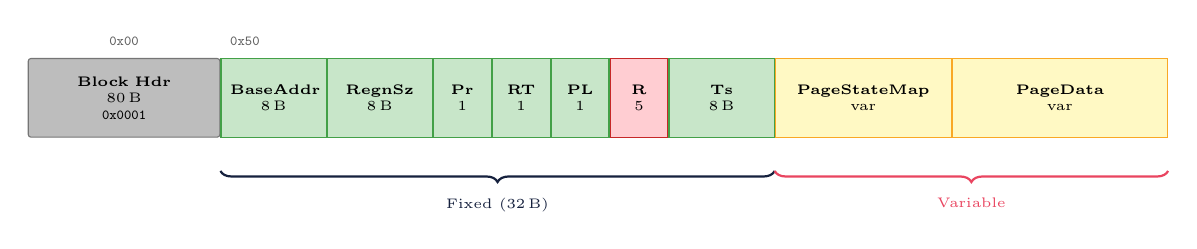
\begin{tikzpicture}[fld/.style={draw, minimum height=1.0cm, align=center, font=\tiny},lbl/.style={font=\tiny\ttfamily, color=muted}]
\node[fld, text width=2.2cm, fill=hdrBox, draw=hdrBoxB, rounded corners=1pt] (hdr) at (0,0) {\textbf{Block Hdr}\\80\,B\\\tiny\texttt{0x0001}};
\node[fld, text width=1.1cm, fill=fldData, draw=fldDataB, right=0pt of hdr] (ba) {\textbf{BaseAddr}\\8\,B};
\node[fld, text width=1.1cm, fill=fldData, draw=fldDataB, right=0pt of ba] (rs) {\textbf{RegnSz}\\8\,B};
\node[fld, text width=0.5cm, fill=fldData, draw=fldDataB, right=0pt of rs] (pr) {\textbf{Pr}\\1};
\node[fld, text width=0.5cm, fill=fldData, draw=fldDataB, right=0pt of pr] (rt) {\textbf{RT}\\1};
\node[fld, text width=0.5cm, fill=fldData, draw=fldDataB, right=0pt of rt] (pl) {\textbf{PL}\\1};
\node[fld, text width=0.5cm, fill=colReserved, draw=colReservedB, right=0pt of pl] (r1) {\textbf{R}\\5};
\node[fld, text width=1.1cm, fill=fldData, draw=fldDataB, right=0pt of r1] (ts) {\textbf{Ts}\\8\,B};
\node[fld, text width=2.0cm, fill=fldVar, draw=fldVarB, right=0pt of ts] (psm) {\textbf{PageStateMap}\\var};
\node[fld, text width=2.5cm, fill=hdrPayload, draw=hdrPayloadB, right=0pt of psm] (pd) {\textbf{PageData}\\var};
\node[lbl, above=1pt of hdr.north] {\hex{00}}; \node[lbl, above=1pt of ba.north west, anchor=south west] {\hex{50}};
\draw[decorate, decoration={brace, amplitude=4pt, mirror, raise=12pt}, thick, color=navy] (ba.south west)--(ts.south east) node[midway, below=18pt, font=\tiny\color{navy}] {Fixed (32\,B)};
\draw[decorate, decoration={brace, amplitude=4pt, mirror, raise=12pt}, thick, color=accent] (psm.south west)--(pd.south east) node[midway, below=18pt, font=\tiny\color{accent}] {Variable};
\end{tikzpicture}}\caption{Memory Region (\hex{0001}). Abbreviations per Table~\ref{tab:memregion}.}\label{fig:memregion-payload}\end{figure}

\subsection{Module Entry (\hex{0002})}\label{sec:modentry}
Stores the identity and metadata of a loaded library (DLL, .so): file path, version string, on-disk hash, and OS-native loader data. \field{ParentUUID} \MUST{} reference the Module List Index (\hex{0010}). \field{BlockUUID} \MUST{} match the pre-assigned \field{ModuleUUID} from the manifest.

\begin{table}[H]\centering\caption{Module Entry payload.}\label{tab:modentry}\small
\begin{tabular}{M M l l p{4cm}}\toprule\textbf{Off}&\textbf{Size}&\textbf{Field}&\textbf{Abbr}&\textbf{Description}\\\midrule
+0x00 & 8 & \field{BaseAddr} & --- & Load address. \\
+0x08 & 8 & \field{ModuleSize} & ModSz & Mapping size. \\
+0x10 & 2 & \field{PathLen} & PL & Path length (incl.\ null, before padding). \\
+0x12 & 2 & \field{VersionLen} & VL & Version length. 0 if unavailable. \\
+0x14 & 4 & \field{Reserved} & R & Zero. \\
+0x18 & var & \field{Path} & --- & UTF-8, pad8. \\
$+p$ & var & \field{Version} & --- & UTF-8, pad8. \\
$+v$ & 32 & \field{DiskHash} & --- & \blake{} of on-disk binary. 32 zero bytes if unavailable. \\
$+v{+}32$ & 4 & \field{BlobLen} & BL & NativeBlob size. \\
$+v{+}36$ & 4 & \field{Reserved2} & R & Zero. \\
$+v{+}40$ & var & \field{NativeBlob} & --- & OS-native opaque data. \\\bottomrule
\end{tabular}\end{table}

\begin{figure}[H]\centering
\resizebox{\textwidth}{!}{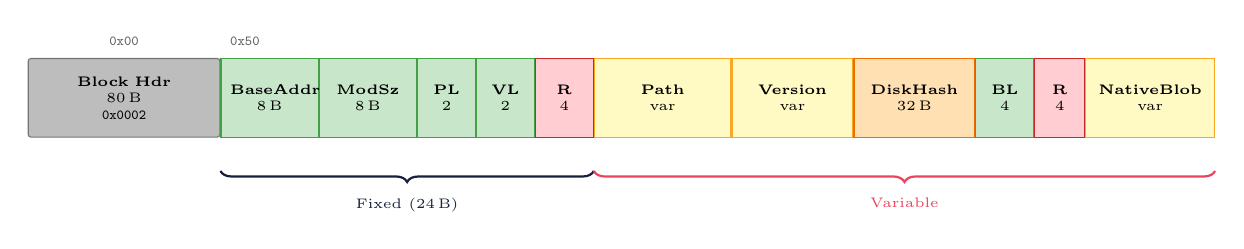
\begin{tikzpicture}[fld/.style={draw, minimum height=1.0cm, align=center, font=\tiny},lbl/.style={font=\tiny\ttfamily, color=muted}]
\node[fld, text width=2.2cm, fill=hdrBox, draw=hdrBoxB, rounded corners=1pt] (hdr) at (0,0) {\textbf{Block Hdr}\\80\,B\\\tiny\texttt{0x0002}};
\node[fld, text width=1.0cm, fill=fldData, draw=fldDataB, right=0pt of hdr] (ba) {\textbf{BaseAddr}\\8\,B};
\node[fld, text width=1.0cm, fill=fldData, draw=fldDataB, right=0pt of ba] (ms) {\textbf{ModSz}\\8\,B};
\node[fld, text width=0.5cm, fill=fldData, draw=fldDataB, right=0pt of ms] (pl) {\textbf{PL}\\2};
\node[fld, text width=0.5cm, fill=fldData, draw=fldDataB, right=0pt of pl] (vl) {\textbf{VL}\\2};
\node[fld, text width=0.5cm, fill=colReserved, draw=colReservedB, right=0pt of vl] (r) {\textbf{R}\\4};
\node[fld, text width=1.5cm, fill=hdrPayload, draw=hdrPayloadB, right=0pt of r] (path) {\textbf{Path}\\var};
\node[fld, text width=1.3cm, fill=fldVar, draw=fldVarB, right=0pt of path] (ver) {\textbf{Version}\\var};
\node[fld, text width=1.3cm, fill=fldCrypto, draw=fldCryptoB, right=0pt of ver] (dh) {\textbf{DiskHash}\\32\,B};
\node[fld, text width=0.5cm, fill=fldData, draw=fldDataB, right=0pt of dh] (bl) {\textbf{BL}\\4};
\node[fld, text width=0.4cm, fill=colReserved, draw=colReservedB, right=0pt of bl] (r2) {\textbf{R}\\4};
\node[fld, text width=1.4cm, fill=fldVar, draw=fldVarB, right=0pt of r2] (nb) {\textbf{NativeBlob}\\var};
\node[lbl, above=1pt of hdr.north] {\hex{00}}; \node[lbl, above=1pt of ba.north west, anchor=south west] {\hex{50}};
\draw[decorate, decoration={brace, amplitude=4pt, mirror, raise=12pt}, thick, color=navy] (ba.south west)--(r.south east) node[midway, below=18pt, font=\tiny\color{navy}] {Fixed (24\,B)};
\draw[decorate, decoration={brace, amplitude=4pt, mirror, raise=12pt}, thick, color=accent] (path.south west)--(nb.south east) node[midway, below=18pt, font=\tiny\color{accent}] {Variable};
\end{tikzpicture}}\caption{Module Entry (\hex{0002}). Abbreviations per Table~\ref{tab:modentry}.}\label{fig:modentry-payload}\end{figure}

\subsection{Module List Index (\hex{0010})}\label{sec:modlist}
\MUST{} be Block~1. Pre-generates UUIDv4 for each Module Entry block.

\begin{table}[H]\centering\caption{Module List Index payload.}\label{tab:modlistentry}\small
\begin{tabular}{M M l l p{4cm}}\toprule\textbf{Off}&\textbf{Size}&\textbf{Field}&\textbf{Abbr}&\textbf{Description}\\\midrule
\multicolumn{5}{l}{\textit{\color{fldPreambleB}--- Preamble ---}} \\
+0x00 & 4 & \field{EntryCount} & ECt & Number of module entries. \\
+0x04 & 4 & \field{Reserved} & R & Zero. \\
\multicolumn{5}{l}{\textit{\color{fldDataB}--- Entry (repeated $\times$\field{EntryCount}), offsets relative to entry start ---}} \\
+0x00 & 16 & \field{ModuleUUID} & ModUUID & Pre-assigned \field{BlockUUID}. \\
+0x10 & 8 & \field{BaseAddr} & --- & Module load address. \\
+0x18 & 8 & \field{ModuleSize} & ModSz & Mapping size. \\
+0x20 & 2 & \field{PathLen} & PL & Path length (incl.\ null). \\
+0x22 & 2 & \field{Reserved} & R & Zero. \\
+0x24 & 4 & \field{Reserved2} & R & Zero. \\
+0x28 & var & \field{Path} & --- & UTF-8, pad8. \\\bottomrule
\end{tabular}\end{table}

\begin{figure}[H]\centering
\resizebox{\textwidth}{!}{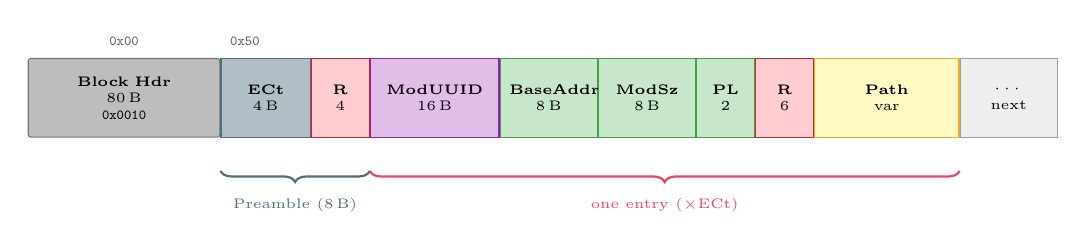
\begin{tikzpicture}[fld/.style={draw, minimum height=1.0cm, align=center, font=\tiny},lbl/.style={font=\tiny\ttfamily, color=muted}]
\node[fld, text width=2.2cm, fill=hdrBox, draw=hdrBoxB, rounded corners=1pt] (hdr) at (0,0) {\textbf{Block Hdr}\\80\,B\\\tiny\texttt{0x0010}};
\node[fld, text width=0.9cm, fill=fldPreamble, draw=fldPreambleB, right=0pt of hdr] (ec) {\textbf{ECt}\\4\,B};
\node[fld, text width=0.5cm, fill=colReserved, draw=colReservedB, right=0pt of ec] (r) {\textbf{R}\\4};
\node[fld, text width=1.4cm, fill=fldUUID, draw=fldUUIDB, right=0pt of r] (mu) {\textbf{ModUUID}\\16\,B};
\node[fld, text width=1.0cm, fill=fldData, draw=fldDataB, right=0pt of mu] (ba) {\textbf{BaseAddr}\\8\,B};
\node[fld, text width=1.0cm, fill=fldData, draw=fldDataB, right=0pt of ba] (ms) {\textbf{ModSz}\\8\,B};
\node[fld, text width=0.5cm, fill=fldData, draw=fldDataB, right=0pt of ms] (pl) {\textbf{PL}\\2};
\node[fld, text width=0.5cm, fill=colReserved, draw=colReservedB, right=0pt of pl] (r2) {\textbf{R}\\6};
\node[fld, text width=1.6cm, fill=hdrPayload, draw=hdrPayloadB, right=0pt of r2] (path) {\textbf{Path}\\var};
\node[fld, text width=1.0cm, fill=fldMore, draw=fldMoreB, right=0pt of path] (more) {$\cdots$\\next};
\node[lbl, above=1pt of hdr.north] {\hex{00}}; \node[lbl, above=1pt of ec.north west, anchor=south west] {\hex{50}};
\draw[decorate, decoration={brace, amplitude=4pt, mirror, raise=12pt}, thick, color=fldPreambleB] (ec.south west)--(r.south east) node[midway, below=18pt, font=\tiny\color{fldPreambleB}] {Preamble (8\,B)};
\draw[decorate, decoration={brace, amplitude=4pt, mirror, raise=12pt}, thick, color=accent] (mu.south west)--(path.south east) node[midway, below=18pt, font=\tiny\color{accent}] {one entry ($\times$ECt)};
\end{tikzpicture}}\caption{Module List Index (\hex{0010}). Abbreviations per Table~\ref{tab:modlistentry}.}\label{fig:modlist-payload}\end{figure}

\subsection{Process Identity (\hex{0040})}\label{sec:procident}
\MUST{} be Block~0 for live acquisition (or after Import Provenance for imports).

\begin{table}[H]\centering\caption{Process Identity payload.}\label{tab:procident}\small
\begin{tabular}{M M l l p{4cm}}\toprule\textbf{Off}&\textbf{Size}&\textbf{Field}&\textbf{Abbr}&\textbf{Description}\\\midrule
+0x00 & 4 & \field{PPID} & --- & Parent PID. 0 if unknown. \\
+0x04 & 4 & \field{SessionID} & SID & 0 if unknown. \\
+0x08 & 8 & \field{StartTime} & StartTm & Process start time. 0 if unknown. \\
+0x10 & 2 & \field{ExePathLen} & EPL & Incl.\ null. \\
+0x12 & 2 & \field{CmdLineLen} & CLL & 0 if unavailable. \\
+0x14 & 4 & \field{Reserved} & R & Zero. \\
+0x18 & var & \field{ExePath} & --- & UTF-8, pad8. \\
$+e$ & var & \field{CmdLine} & --- & UTF-8, pad8. \\\bottomrule
\end{tabular}\end{table}

\begin{figure}[H]\centering
\resizebox{\textwidth}{!}{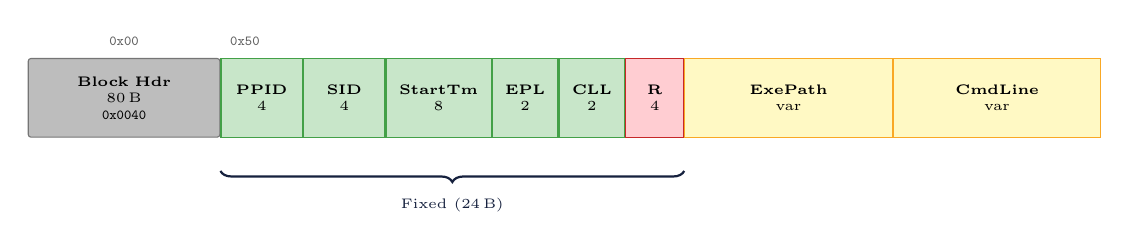
\begin{tikzpicture}[fld/.style={draw, minimum height=1.0cm, align=center, font=\tiny},lbl/.style={font=\tiny\ttfamily, color=muted}]
\node[fld, text width=2.2cm, fill=hdrBox, draw=hdrBoxB, rounded corners=1pt] (hdr) at (0,0) {\textbf{Block Hdr}\\80\,B\\\tiny\texttt{0x0040}};
\node[fld, text width=0.8cm, fill=fldData, draw=fldDataB, right=0pt of hdr] (ppid) {\textbf{PPID}\\4};
\node[fld, text width=0.8cm, fill=fldData, draw=fldDataB, right=0pt of ppid] (sid) {\textbf{SID}\\4};
\node[fld, text width=1.1cm, fill=fldData, draw=fldDataB, right=0pt of sid] (st) {\textbf{StartTm}\\8};
\node[fld, text width=0.6cm, fill=fldData, draw=fldDataB, right=0pt of st] (epl) {\textbf{EPL}\\2};
\node[fld, text width=0.6cm, fill=fldData, draw=fldDataB, right=0pt of epl] (cll) {\textbf{CLL}\\2};
\node[fld, text width=0.5cm, fill=colReserved, draw=colReservedB, right=0pt of cll] (r) {\textbf{R}\\4};
\node[fld, text width=2.4cm, fill=hdrPayload, draw=hdrPayloadB, right=0pt of r] (ep) {\textbf{ExePath}\\var};
\node[fld, text width=2.4cm, fill=fldVar, draw=fldVarB, right=0pt of ep] (cl) {\textbf{CmdLine}\\var};
\node[lbl, above=1pt of hdr.north] {\hex{00}}; \node[lbl, above=1pt of ppid.north west, anchor=south west] {\hex{50}};
\draw[decorate, decoration={brace, amplitude=4pt, mirror, raise=12pt}, thick, color=navy] (ppid.south west)--(r.south east) node[midway, below=18pt, font=\tiny\color{navy}] {Fixed (24\,B)};
\end{tikzpicture}}\caption{Process Identity (\hex{0040}). Abbreviations per Table~\ref{tab:procident}.}\label{fig:procident-payload}\end{figure}

\subsection{Related Dump (\hex{0041})}\label{sec:relateddump}
An acquirer \MAY{} emit one or more Related Dump blocks to record relationships between concurrently captured processes (parent/child, shared-memory peers, IPC partners).

\begin{table}[H]\centering\caption{Related Dump payload (24 bytes, fixed).}\label{tab:relateddump}\small
\begin{tabular}{M M l l p{4cm}}\toprule\textbf{Off}&\textbf{Size}&\textbf{Field}&\textbf{Abbr}&\textbf{Description}\\\midrule
+0x00 & 16 & \field{RelatedDumpUUID} & RelDumpUUID & \field{DumpUUID} of related file. \\
+0x10 & 4 & \field{RelatedPID} & RelPID & 0 if unknown. \\
+0x14 & 2 & \field{Relationship} & Rel & \hex{0001}=Parent, \hex{0002}=Child, \hex{0003}=SharedMemory, \hex{0004}=IPC peer, \hex{0005}=Thread group, \hex{FFFF}=Other. \\
+0x16 & 2 & \field{Reserved} & R & Zero. \\\bottomrule
\end{tabular}\end{table}

\begin{figure}[H]\centering
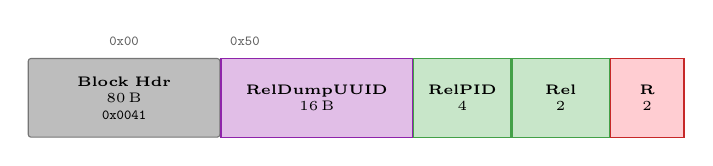
\begin{tikzpicture}[fld/.style={draw, minimum height=1.0cm, align=center, font=\tiny},lbl/.style={font=\tiny\ttfamily, color=muted}]
\node[fld, text width=2.2cm, fill=hdrBox, draw=hdrBoxB, rounded corners=1pt] (hdr) at (0,0) {\textbf{Block Hdr}\\80\,B\\\tiny\texttt{0x0041}};
\node[fld, text width=2.2cm, fill=fldUUID, draw=fldUUIDB, right=0pt of hdr] (ru) {\textbf{RelDumpUUID}\\16\,B};
\node[fld, text width=1.0cm, fill=fldData, draw=fldDataB, right=0pt of ru] (rp) {\textbf{RelPID}\\4};
\node[fld, text width=1.0cm, fill=fldData, draw=fldDataB, right=0pt of rp] (rel) {\textbf{Rel}\\2};
\node[fld, text width=0.7cm, fill=colReserved, draw=colReservedB, right=0pt of rel] (r) {\textbf{R}\\2};
\node[lbl, above=1pt of hdr.north] {\hex{00}}; \node[lbl, above=1pt of ru.north west, anchor=south west] {\hex{50}};
\end{tikzpicture}
\caption{Related Dump (\hex{0041}). Abbreviations per Table~\ref{tab:relateddump}.}\label{fig:relateddump-payload}\end{figure}

\subsection{Key Hint (\hex{0020})}\label{sec:keyhint}
A Key Hint block annotates a region of captured memory that is believed to contain cryptographic key material. It records the key's location (via \field{RegionUUID} and byte offset), its type and protocol association, and a confidence level reflecting how the key was identified (speculative scan, heuristic match, or confirmed via instrumentation). Key Hints are \OPTIONAL; their presence is indicated by the \field{CryptoHints} bit in \field{CapBitmap} and the \field{HasKeyHints} flag on the referenced Memory Region block.

\begin{table}[H]\centering\caption{Key Hint payload.}\label{tab:keyhint}\small
\begin{tabular}{M M l l p{4cm}}\toprule\textbf{Off}&\textbf{Size}&\textbf{Field}&\textbf{Abbr}&\textbf{Description}\\\midrule
+0x00 & 16 & \field{RegionUUID} & RgnUUID & Memory Region \field{BlockUUID}. \\
+0x10 & 8 & \field{RegionOffset} & RgnOff & Byte offset in \field{PageData}. \\
+0x18 & 4 & \field{KeyLen} & KLen & 0 if unknown. \\
+0x1C & 2 & \field{KeyType} & KT & Table~\ref{tab:keytypes}. \\
+0x1E & 2 & \field{Protocol} & Pr & Table~\ref{tab:keytypes}. \\
+0x20 & 1 & \field{Confidence} & C & \hex{00}=Speculative, \hex{01}=Heuristic, \hex{02}=Confirmed. \\
+0x21 & 1 & \field{KeyState} & S & \hex{00}=Unknown, \hex{01}=Active, \hex{02}=Expired. \\
+0x22 & 2 & \field{Reserved} & R & Zero. \\
+0x24 & 4 & \field{NoteLen} & NL & 0 if none. \\
+0x28 & 4 & \field{Reserved2} & R & Zero. \\
+0x2C & var & \field{Note} & --- & UTF-8, pad8. \\\bottomrule
\end{tabular}\end{table}

\begin{figure}[H]\centering
\resizebox{\textwidth}{!}{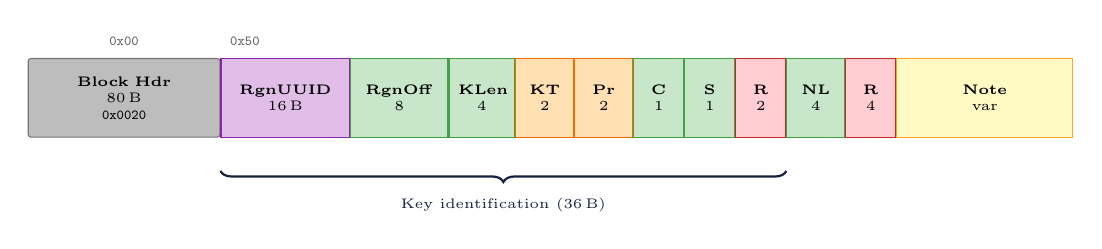
\begin{tikzpicture}[fld/.style={draw, minimum height=1.0cm, align=center, font=\tiny},lbl/.style={font=\tiny\ttfamily, color=muted}]
\node[fld, text width=2.2cm, fill=hdrBox, draw=hdrBoxB, rounded corners=1pt] (hdr) at (0,0) {\textbf{Block Hdr}\\80\,B\\\tiny\texttt{0x0020}};
\node[fld, text width=1.4cm, fill=fldUUID, draw=fldUUIDB, right=0pt of hdr] (ru) {\textbf{RgnUUID}\\16\,B};
\node[fld, text width=1.0cm, fill=fldData, draw=fldDataB, right=0pt of ru] (ro) {\textbf{RgnOff}\\8};
\node[fld, text width=0.6cm, fill=fldData, draw=fldDataB, right=0pt of ro] (kl) {\textbf{KLen}\\4};
\node[fld, text width=0.5cm, fill=fldCrypto, draw=fldCryptoB, right=0pt of kl] (kt) {\textbf{KT}\\2};
\node[fld, text width=0.5cm, fill=fldCrypto, draw=fldCryptoB, right=0pt of kt] (pr) {\textbf{Pr}\\2};
\node[fld, text width=0.4cm, fill=fldData, draw=fldDataB, right=0pt of pr] (cf) {\textbf{C}\\1};
\node[fld, text width=0.4cm, fill=fldData, draw=fldDataB, right=0pt of cf] (ks) {\textbf{S}\\1};
\node[fld, text width=0.4cm, fill=colReserved, draw=colReservedB, right=0pt of ks] (r1) {\textbf{R}\\2};
\node[fld, text width=0.5cm, fill=fldData, draw=fldDataB, right=0pt of r1] (nl) {\textbf{NL}\\4};
\node[fld, text width=0.4cm, fill=colReserved, draw=colReservedB, right=0pt of nl] (r2) {\textbf{R}\\4};
\node[fld, text width=2.0cm, fill=fldVar, draw=fldVarB, right=0pt of r2] (note) {\textbf{Note}\\var};
\node[lbl, above=1pt of hdr.north] {\hex{00}}; \node[lbl, above=1pt of ru.north west, anchor=south west] {\hex{50}};
\draw[decorate, decoration={brace, amplitude=4pt, mirror, raise=12pt}, thick, color=navy] (ru.south west)--(r1.south east) node[midway, below=18pt, font=\tiny\color{navy}] {Key identification (36\,B)};
\end{tikzpicture}}\caption{Key Hint (\hex{0020}). Abbreviations per Table~\ref{tab:keyhint}.}\label{fig:keyhint-payload}\end{figure}

\begin{table}[H]\centering\caption{Key type and protocol codes.}\label{tab:keytypes}\small
\begin{minipage}[t]{0.46\textwidth}\centering\subcaption*{\textbf{Key type codes} (\field{KeyType})}
\begin{tabular}{M l}\toprule\textbf{Code}&\textbf{Type}\\\midrule
0x0000 & Unknown \\ 0x0001 & Pre-Master Secret \\ 0x0002 & Master Secret \\ 0x0003 & Session Key \\ 0x0004 & Handshake Secret \\ 0x0005 & App Traffic Secret \\ 0x0006 & RSA Private Key \\ 0x0007 & ECDH Private Key \\ 0x0008 & IKE SA Key \\ 0x0009 & ESP/AH Key \\ 0x000A & SSH Session Key \\ 0x000B & WireGuard Key \\ 0x000C & ML-KEM Private Key \\ 0xFFFF & Other \\\bottomrule
\end{tabular}\end{minipage}%
\hfill
\begin{minipage}[t]{0.46\textwidth}\centering\subcaption*{\textbf{Protocol codes} (\field{Protocol})}
\begin{tabular}{M l}\toprule\textbf{Code}&\textbf{Protocol}\\\midrule
0x0000 & Unknown \\ 0x0001 & TLS 1.2 \\ 0x0002 & TLS 1.3 \\ 0x0003 & DTLS 1.2 \\ 0x0004 & DTLS 1.3 \\ 0x0005 & QUIC \\ 0x0006 & IKEv2/IPsec \\ 0x0007 & SSH \\ 0x0008 & WireGuard \\ 0x0009 & PQ-TLS (hybrid) \\ 0xFFFF & Other \\\bottomrule
\end{tabular}\end{minipage}
\end{table}

%% ======================================================================
\newpage
\section{Investigation Mode}\label{sec:investigation}
%% ======================================================================
When \field{Investigation} (bit~1) is set, the acquirer \MUST{} capture system-wide context alongside per-process memory: acquisition operator, system hostname, and system-wide tables (process list, network connections, open handles). When not set, the acquisition is in Analysis mode and \MUST{} follow Figure~\ref{fig:acq-sequence}.

\subsection{Block Ordering}
\begin{enumerate}[leftmargin=1.8em, itemsep=2pt]
\item \textbf{Block~0:} Process Identity (\hex{0040}).
\item \textbf{Block~1:} Module List Index (\hex{0010}).
\item \textbf{Block~2:} System Context (\hex{0050}) --- \REQUIRED.
\end{enumerate}
System-wide table blocks (\hex{0051}--\hex{0053}) follow with \field{ParentUUID} referencing the System Context block.

\begin{figure}[H]\centering
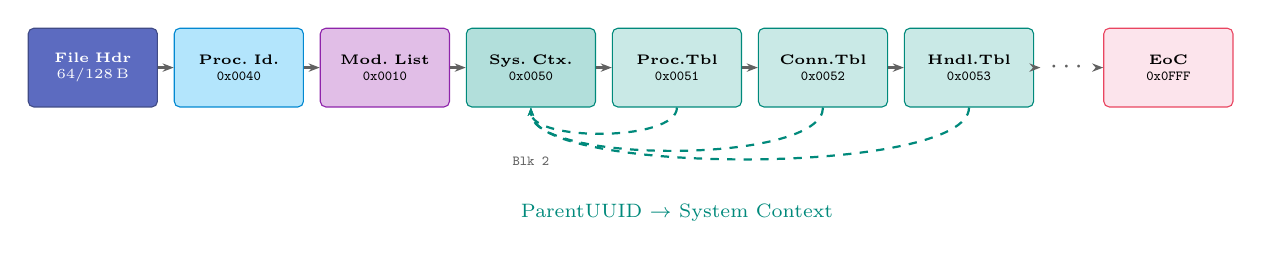
\begin{tikzpicture}[blk/.style={draw, rounded corners=2pt, minimum height=1.0cm, text width=1.5cm, align=center, inner sep=2pt, font=\tiny},lbl/.style={font=\tiny\ttfamily, color=muted},arr/.style={-{Stealth[length=4pt]}, thick, color=muted}]
\node[blk, fill=btFileHdr, draw=btFileHdr!70!black, text=white] (hdr) at (0,0) {\textbf{File Hdr}\\64/128\,B};
\node[blk, fill=btProcIdent, draw=btProcIdentB, right=0.2cm of hdr] (b0) {\textbf{Proc.\ Id.}\\\hex{0040}};
\node[blk, fill=btModule, draw=btModuleB, right=0.2cm of b0] (b1) {\textbf{Mod.\ List}\\\hex{0010}};
\node[blk, fill=btSysCtx, draw=btSysCtxB, right=0.2cm of b1] (b2) {\textbf{Sys.\ Ctx.}\\\hex{0050}};
\node[blk, fill=btSysTable!70, draw=btSysCtxB, right=0.2cm of b2] (b3) {\textbf{Proc.Tbl}\\\hex{0051}};
\node[blk, fill=btSysTable!70, draw=btSysCtxB, right=0.2cm of b3] (b4) {\textbf{Conn.Tbl}\\\hex{0052}};
\node[blk, fill=btSysTable!70, draw=btSysCtxB, right=0.2cm of b4] (b5) {\textbf{Hndl.Tbl}\\\hex{0053}};
\node[right=0.08cm of b5, font=\normalsize\bfseries, color=muted] (dots) {$\cdots$};
\node[blk, fill=btEoC, draw=btEoCB, right=0.08cm of dots] (eoc) {\textbf{EoC}\\\hex{0FFF}};
\draw[arr] (hdr)--(b0); \draw[arr] (b0)--(b1); \draw[arr] (b1)--(b2); \draw[arr] (b2)--(b3); \draw[arr] (b3)--(b4); \draw[arr] (b4)--(b5); \draw[arr] (b5)--(dots); \draw[arr] (dots)--(eoc);
\node[lbl, below=0.5cm of b2.south] {Blk 2};
\draw[-{Stealth[length=3pt]}, thick, dashed, color=btSysCtxB] (b3.south) to[out=-90, in=-90, looseness=0.6] (b2.south);
\draw[-{Stealth[length=3pt]}, thick, dashed, color=btSysCtxB] (b4.south) to[out=-90, in=-90, looseness=0.5] (b2.south);
\draw[-{Stealth[length=3pt]}, thick, dashed, color=btSysCtxB] (b5.south) to[out=-90, in=-90, looseness=0.4] (b2.south);
\node[font=\scriptsize\color{btSysCtxB}, below=1.1cm of b3.south] {ParentUUID $\to$ System Context};
\end{tikzpicture}
\caption{Investigation mode block sequence. System table blocks reference System Context via \field{ParentUUID}.}\label{fig:inv-sequence}\end{figure}

\subsection{System Context Block (\hex{0050})}\label{sec:sysctx}
The System Context block captures system-wide metadata at acquisition time: the identity of the acquisition operator, the target system's hostname and OS version, and a bitmap indicating which system-wide table blocks (\hex{0051}--\hex{0053}) are present. This block \MUST{} be Block~2 when \field{Investigation} is set. The \field{TableBitmap} allows consumers to determine which tables to expect without scanning ahead.

\begin{table}[H]\centering\caption{System Context payload.}\label{tab:sysctx}\small
\begin{tabular}{M M l l p{3.5cm}}\toprule\textbf{Off}&\textbf{Size}&\textbf{Field}&\textbf{Abbr}&\textbf{Description}\\\midrule
+0x00 & 8 & \field{BootTime} & BootTm & System boot time. 0 if unknown. \\
+0x08 & 4 & \field{TargetCount} & TCt & Processes targeted this session. \\
+0x0C & 4 & \field{TableBitmap} & TBm & Bit~0=ProcessTable, 1=ConnectionTable, 2=HandleTable. \\
+0x10 & 2 & \field{AcqUserLen} & --- & Incl.\ null. \\
+0x12 & 2 & \field{HostnameLen} & --- & Incl.\ null. \\
+0x14 & 2 & \field{DomainLen} & --- & 0 if N/A. \\
+0x16 & 2 & \field{OSDetailLen} & --- & \\
+0x18 & 2 & \field{CaseRefLen} & --- & 0 if none. \\
+0x1A & 6 & \field{Reserved} & R & Zero. \\
+0x20 & var & \field{AcqUser} & --- & UTF-8, pad8. Acquisition operator. \\
$+u$ & var & \field{Hostname} & --- & UTF-8, pad8. \\
$+h$ & var & \field{Domain} & --- & UTF-8, pad8. Omitted if len=0. \\
$+d$ & var & \field{OSDetail} & OSDet & UTF-8, pad8. \\
$+o$ & var & \field{CaseRef} & --- & UTF-8, pad8. Omitted if len=0. \\\bottomrule
\end{tabular}\end{table}

The \field{TableBitmap} field advertises which tables and system-context
extension blocks are present in the slice. Each bit is associated with a
single block identifier, so that a reader can derive the expected block
inventory directly from the SystemContext block rather than by scanning
the slice. Bit assignments are listed in Table~\ref{tab:sysctx-bitmap};
bits~10--31 are reserved and shall be emitted as zero.

\begin{table}[H]\centering\caption{\field{TableBitmap} bit assignments.}\label{tab:sysctx-bitmap}\small
\begin{tabular}{c l l p{5.5cm}}\toprule
\textbf{Bit} & \textbf{Mask} & \textbf{Block} & \textbf{Set when} \\\midrule
0 & 0x0001 & \field{ProcessTable} (\texttt{0x0051}) & The system process table is emitted. \\
1 & 0x0002 & \field{ConnectionTable} (\texttt{0x0052}) & The system socket-connection table is emitted. \\
2 & 0x0004 & \field{HandleTable} (\texttt{0x0053}) & The per-target handle table is emitted. \\
3 & 0x0008 & \field{ConnectivityTable} (\texttt{0x0054}) & The collector produced at least one row of kernel network state (routes, ARP, packet sockets, interface counters, socket-family aggregates, or MIB counters). \\

\bottomrule
\end{tabular}\end{table}

\begin{figure}[H]\centering
\resizebox{\textwidth}{!}{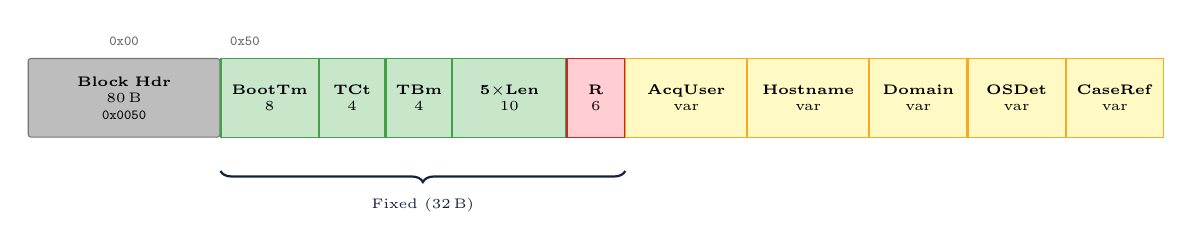
\begin{tikzpicture}[fld/.style={draw, minimum height=1.0cm, align=center, font=\tiny},lbl/.style={font=\tiny\ttfamily, color=muted}]
\node[fld, text width=2.2cm, fill=hdrBox, draw=hdrBoxB, rounded corners=1pt] (hdr) at (0,0) {\textbf{Block Hdr}\\80\,B\\\tiny\texttt{0x0050}};
\node[fld, text width=1.0cm, fill=fldData, draw=fldDataB, right=0pt of hdr] (bt) {\textbf{BootTm}\\8};
\node[fld, text width=0.6cm, fill=fldData, draw=fldDataB, right=0pt of bt] (tc) {\textbf{TCt}\\4};
\node[fld, text width=0.6cm, fill=fldData, draw=fldDataB, right=0pt of tc] (tb) {\textbf{TBm}\\4};
\node[fld, text width=1.2cm, fill=fldData, draw=fldDataB, right=0pt of tb] (lens) {\textbf{5$\times$Len}\\10};
\node[fld, text width=0.5cm, fill=colReserved, draw=colReservedB, right=0pt of lens] (r) {\textbf{R}\\6};
\node[fld, text width=1.3cm, fill=hdrPayload, draw=hdrPayloadB, right=0pt of r] (au) {\textbf{AcqUser}\\var};
\node[fld, text width=1.3cm, fill=hdrPayload, draw=hdrPayloadB, right=0pt of au] (hn) {\textbf{Hostname}\\var};
\node[fld, text width=1.0cm, fill=fldVar, draw=fldVarB, right=0pt of hn] (dm) {\textbf{Domain}\\var};
\node[fld, text width=1.0cm, fill=fldVar, draw=fldVarB, right=0pt of dm] (os) {\textbf{OSDet}\\var};
\node[fld, text width=1.0cm, fill=fldVar, draw=fldVarB, right=0pt of os] (cr) {\textbf{CaseRef}\\var};
\node[lbl, above=1pt of hdr.north] {\hex{00}}; \node[lbl, above=1pt of bt.north west, anchor=south west] {\hex{50}};
\draw[decorate, decoration={brace, amplitude=4pt, mirror, raise=12pt}, thick, color=navy] (bt.south west)--(r.south east) node[midway, below=18pt, font=\tiny\color{navy}] {Fixed (32\,B)};
\end{tikzpicture}}\caption{System Context (\hex{0050}). Abbreviations per Table~\ref{tab:sysctx}.}\label{fig:sysctx-layout}\end{figure}

The block definitions that follow specify the system-context metadata classes in the identifier range \texttt{0x0051}--\texttt{0x0054}. Each block is additive: readers that do not recognize a block type skip it according to the rules of Section~\ref{sec:blocks}, and the format therefore remains forward compatible. Presence is advertised through a dedicated bit in the SystemContext \field{TableBitmap} (Table~\ref{tab:sysctx-bitmap}).

\subsection{Process Table (\hex{0051})}\label{sec:proctable}
System-wide process snapshot. \field{ParentUUID} \MUST{} reference the System Context block.

\begin{table}[H]\centering\caption{Process Table payload.}\label{tab:procentry}\small
\begin{tabular}{M M l l p{3.5cm}}\toprule\textbf{Off}&\textbf{Size}&\textbf{Field}&\textbf{Abbr}&\textbf{Description}\\\midrule
\multicolumn{5}{l}{\textit{\color{fldPreambleB}--- Preamble ---}} \\
+0x00 & 4 & \field{EntryCount} & ECt & Number of process entries. \\
+0x04 & 4 & \field{Reserved} & R & Zero. \\
\multicolumn{5}{l}{\textit{\color{fldDataB}--- Entry (repeated $\times$\field{EntryCount}), offsets relative to entry start ---}} \\
+0x00 & 4 & \field{PID} & --- & \\ +0x04 & 4 & \field{PPID} & --- & Parent PID. \\
+0x08 & 4 & \field{UID} & --- & POSIX UID or SID hash. \\
+0x0C & 1 & \field{IsTarget} & T & \hex{01} if acquisition target. \\
+0x0D & 3 & \field{Reserved} & R & Zero. \\
+0x10 & 8 & \field{StartTime} & StTm & 0 if unknown. \\
+0x18 & 8 & \field{RSS} & --- & 0 if unknown. \\
+0x20 & 2 & \field{ExeNameLen} & --- & Incl.\ null. \\
+0x22 & 2 & \field{CmdLineLen} & --- & 0 if unavailable. \\
+0x24 & 2 & \field{UserLen} & --- & 0 if unavailable. \\
+0x26 & 2 & \field{Reserved2} & R & Zero. \\
+0x28 & var & \field{ExeName} & --- & UTF-8, pad8. \\
$+e$ & var & \field{CmdLine} & --- & UTF-8, pad8. \\
$+c$ & var & \field{User} & --- & UTF-8, pad8. \\\bottomrule
\end{tabular}\end{table}

\begin{figure}[H]\centering
\resizebox{\textwidth}{!}{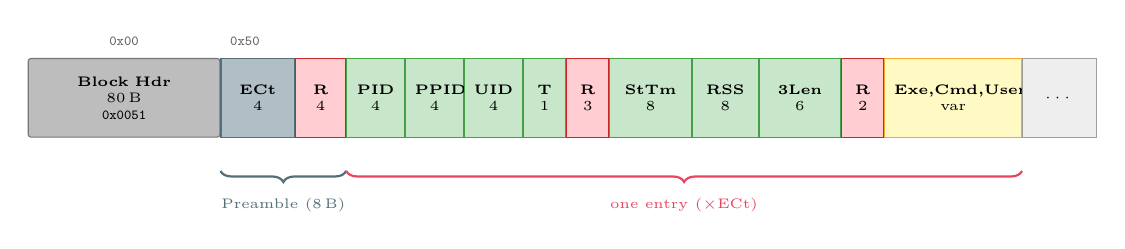
\begin{tikzpicture}[fld/.style={draw, minimum height=1.0cm, align=center, font=\tiny},lbl/.style={font=\tiny\ttfamily, color=muted}]
\node[fld, text width=2.2cm, fill=hdrBox, draw=hdrBoxB, rounded corners=1pt] (hdr) at (0,0) {\textbf{Block Hdr}\\80\,B\\\tiny\texttt{0x0051}};
\node[fld, text width=0.7cm, fill=fldPreamble, draw=fldPreambleB, right=0pt of hdr] (ec) {\textbf{ECt}\\4};
\node[fld, text width=0.4cm, fill=colReserved, draw=colReservedB, right=0pt of ec] (r) {\textbf{R}\\4};
\node[fld, text width=0.5cm, fill=fldData, draw=fldDataB, right=0pt of r] (pid) {\textbf{PID}\\4};
\node[fld, text width=0.5cm, fill=fldData, draw=fldDataB, right=0pt of pid] (ppid) {\textbf{PPID}\\4};
\node[fld, text width=0.5cm, fill=fldData, draw=fldDataB, right=0pt of ppid] (uid) {\textbf{UID}\\4};
\node[fld, text width=0.3cm, fill=fldData, draw=fldDataB, right=0pt of uid] (tgt) {\textbf{T}\\1};
\node[fld, text width=0.3cm, fill=colReserved, draw=colReservedB, right=0pt of tgt] (r2) {\textbf{R}\\3};
\node[fld, text width=0.8cm, fill=fldData, draw=fldDataB, right=0pt of r2] (st) {\textbf{StTm}\\8};
\node[fld, text width=0.6cm, fill=fldData, draw=fldDataB, right=0pt of st] (rss) {\textbf{RSS}\\8};
\node[fld, text width=0.8cm, fill=fldData, draw=fldDataB, right=0pt of rss] (lens) {\textbf{3Len}\\6};
\node[fld, text width=0.3cm, fill=colReserved, draw=colReservedB, right=0pt of lens] (r3) {\textbf{R}\\2};
\node[fld, text width=1.5cm, fill=hdrPayload, draw=hdrPayloadB, right=0pt of r3] (vars) {\textbf{Exe,Cmd,User}\\var};
\node[fld, text width=0.7cm, fill=fldMore, draw=fldMoreB, right=0pt of vars] (more) {$\cdots$};
\node[lbl, above=1pt of hdr.north] {\hex{00}}; \node[lbl, above=1pt of ec.north west, anchor=south west] {\hex{50}};
\draw[decorate, decoration={brace, amplitude=4pt, mirror, raise=12pt}, thick, color=fldPreambleB] (ec.south west)--(r.south east) node[midway, below=18pt, font=\tiny\color{fldPreambleB}] {Preamble (8\,B)};
\draw[decorate, decoration={brace, amplitude=4pt, mirror, raise=12pt}, thick, color=accent] (pid.south west)--(vars.south east) node[midway, below=18pt, font=\tiny\color{accent}] {one entry ($\times$ECt)};
\end{tikzpicture}}\caption{Process Table (\hex{0051}). Abbreviations per Table~\ref{tab:procentry}.}\label{fig:proctable-payload}\end{figure}

\subsection{Connection Table (\hex{0052})}\label{sec:conntable}
System-wide network sockets. \field{ParentUUID} \MUST{} reference System Context.

\begin{notebox}[title={Port byte order}]
\field{LocalPort} and \field{RemotePort} are structural integers and therefore stored as little-endian \texttt{uint16}, regardless of the network byte order (big-endian) used by OS socket APIs. Producers \MUST{} convert from network byte order before writing.
\end{notebox}

\begin{table}[H]\centering\caption{Connection Table payload.}\label{tab:connentry}\small
\begin{tabular}{M M l l p{3.5cm}}\toprule\textbf{Off}&\textbf{Size}&\textbf{Field}&\textbf{Abbr}&\textbf{Description}\\\midrule
\multicolumn{5}{l}{\textit{\color{fldPreambleB}--- Preamble ---}} \\
+0x00 & 4 & \field{EntryCount} & ECt & Number of connection entries. \\
+0x04 & 4 & \field{Reserved} & R & Zero. \\
\multicolumn{5}{l}{\textit{\color{fldDataB}--- Entry (repeated $\times$\field{EntryCount}), 48 bytes fixed, offsets relative to entry start ---}} \\
+0x00 & 4 & \field{PID} & --- & 0 if unknown. \\
+0x04 & 1 & \field{Family} & F & \hex{02}=IPv4, \hex{0A}=IPv6. \\
+0x05 & 1 & \field{Protocol} & P & \hex{06}=TCP, \hex{11}=UDP. \\
+0x06 & 1 & \field{State} & S & TCP state. \hex{00}=N/A. \\
+0x07 & 1 & \field{Reserved} & R & Zero. \\
+0x08 & 16 & \field{LocalAddr} & --- & IPv4: 4B used, rest zero. \\
+0x18 & 2 & \field{LocalPort} & LP & Little-endian \texttt{uint16}. \\
+0x1A & 2 & \field{Reserved2} & R & Zero. \\
+0x1C & 16 & \field{RemoteAddr} & --- & Zeros for LISTEN. \\
+0x2C & 2 & \field{RemotePort} & RP & 0 for LISTEN/UDP. \\
+0x2E & 2 & \field{Reserved3} & R & Zero. \\\bottomrule
\end{tabular}\end{table}

\begin{figure}[H]\centering
\resizebox{\textwidth}{!}{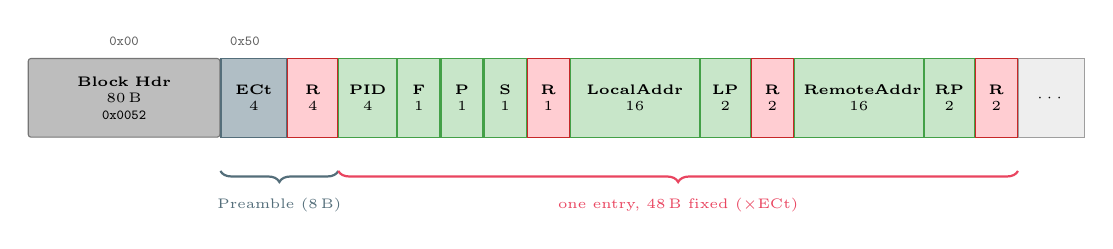
\begin{tikzpicture}[fld/.style={draw, minimum height=1.0cm, align=center, font=\tiny},lbl/.style={font=\tiny\ttfamily, color=muted}]
\node[fld, text width=2.2cm, fill=hdrBox, draw=hdrBoxB, rounded corners=1pt] (hdr) at (0,0) {\textbf{Block Hdr}\\80\,B\\\tiny\texttt{0x0052}};
\node[fld, text width=0.6cm, fill=fldPreamble, draw=fldPreambleB, right=0pt of hdr] (ec) {\textbf{ECt}\\4};
\node[fld, text width=0.4cm, fill=colReserved, draw=colReservedB, right=0pt of ec] (r) {\textbf{R}\\4};
\node[fld, text width=0.5cm, fill=fldData, draw=fldDataB, right=0pt of r] (pid) {\textbf{PID}\\4};
\node[fld, text width=0.3cm, fill=fldData, draw=fldDataB, right=0pt of pid] (fam) {\textbf{F}\\1};
\node[fld, text width=0.3cm, fill=fldData, draw=fldDataB, right=0pt of fam] (proto) {\textbf{P}\\1};
\node[fld, text width=0.3cm, fill=fldData, draw=fldDataB, right=0pt of proto] (st) {\textbf{S}\\1};
\node[fld, text width=0.3cm, fill=colReserved, draw=colReservedB, right=0pt of st] (r2) {\textbf{R}\\1};
\node[fld, text width=1.4cm, fill=fldData, draw=fldDataB, right=0pt of r2] (la) {\textbf{LocalAddr}\\16};
\node[fld, text width=0.4cm, fill=fldData, draw=fldDataB, right=0pt of la] (lp) {\textbf{LP}\\2};
\node[fld, text width=0.3cm, fill=colReserved, draw=colReservedB, right=0pt of lp] (r3) {\textbf{R}\\2};
\node[fld, text width=1.4cm, fill=fldData, draw=fldDataB, right=0pt of r3] (ra) {\textbf{RemoteAddr}\\16};
\node[fld, text width=0.4cm, fill=fldData, draw=fldDataB, right=0pt of ra] (rp) {\textbf{RP}\\2};
\node[fld, text width=0.3cm, fill=colReserved, draw=colReservedB, right=0pt of rp] (r4) {\textbf{R}\\2};
\node[fld, text width=0.6cm, fill=fldMore, draw=fldMoreB, right=0pt of r4] (more) {$\cdots$};
\node[lbl, above=1pt of hdr.north] {\hex{00}}; \node[lbl, above=1pt of ec.north west, anchor=south west] {\hex{50}};
\draw[decorate, decoration={brace, amplitude=4pt, mirror, raise=12pt}, thick, color=fldPreambleB] (ec.south west)--(r.south east) node[midway, below=18pt, font=\tiny\color{fldPreambleB}] {Preamble (8\,B)};
\draw[decorate, decoration={brace, amplitude=4pt, mirror, raise=12pt}, thick, color=accent] (pid.south west)--(r4.south east) node[midway, below=18pt, font=\tiny\color{accent}] {one entry, 48\,B fixed ($\times$ECt)};
\end{tikzpicture}}\caption{Connection Table (\hex{0052}). Abbreviations per Table~\ref{tab:connentry}.}\label{fig:conntable-payload}\end{figure}

\subsection{Handle Table (\hex{0053})}\label{sec:handletable}
System-wide file descriptors/handles. \field{ParentUUID} \MUST{} reference System Context.

\begin{table}[H]\centering\caption{Handle Table payload.}\label{tab:handleentry}\small
\begin{tabular}{M M l l p{3.5cm}}\toprule\textbf{Off}&\textbf{Size}&\textbf{Field}&\textbf{Abbr}&\textbf{Description}\\\midrule
\multicolumn{5}{l}{\textit{\color{fldPreambleB}--- Preamble ---}} \\
+0x00 & 4 & \field{EntryCount} & ECt & Number of handle entries. \\
+0x04 & 4 & \field{Reserved} & R & Zero. \\
\multicolumn{5}{l}{\textit{\color{fldDataB}--- Entry (repeated $\times$\field{EntryCount}), offsets relative to entry start ---}} \\
+0x00 & 4 & \field{PID} & --- & \\ +0x04 & 4 & \field{FD} & --- & Descriptor/handle number. \\
+0x08 & 1 & \field{HandleType} & HT & \hex{00}=Unknown, \hex{01}=File, \hex{02}=Dir, \hex{03}=Socket, \hex{04}=Pipe, \hex{05}=Device, \hex{06}=Registry, \hex{FF}=Other. \\
+0x09 & 1 & \field{Reserved} & R & Zero. \\
+0x0A & 2 & \field{PathLen} & PL & 0 if unavailable. \\
+0x0C & 4 & \field{Reserved2} & R & Zero. \\
+0x10 & var & \field{Path} & --- & UTF-8, pad8. \\\bottomrule
\end{tabular}\end{table}

\begin{figure}[H]\centering
\resizebox{\textwidth}{!}{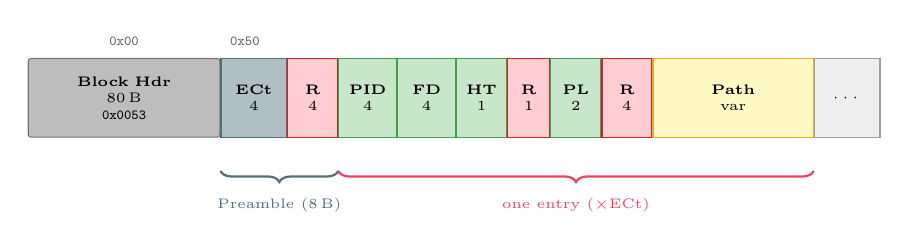
\begin{tikzpicture}[fld/.style={draw, minimum height=1.0cm, align=center, font=\tiny},lbl/.style={font=\tiny\ttfamily, color=muted}]
\node[fld, text width=2.2cm, fill=hdrBox, draw=hdrBoxB, rounded corners=1pt] (hdr) at (0,0) {\textbf{Block Hdr}\\80\,B\\\tiny\texttt{0x0053}};
\node[fld, text width=0.6cm, fill=fldPreamble, draw=fldPreambleB, right=0pt of hdr] (ec) {\textbf{ECt}\\4};
\node[fld, text width=0.4cm, fill=colReserved, draw=colReservedB, right=0pt of ec] (r) {\textbf{R}\\4};
\node[fld, text width=0.5cm, fill=fldData, draw=fldDataB, right=0pt of r] (pid) {\textbf{PID}\\4};
\node[fld, text width=0.5cm, fill=fldData, draw=fldDataB, right=0pt of pid] (fd) {\textbf{FD}\\4};
\node[fld, text width=0.4cm, fill=fldData, draw=fldDataB, right=0pt of fd] (ht) {\textbf{HT}\\1};
\node[fld, text width=0.3cm, fill=colReserved, draw=colReservedB, right=0pt of ht] (r2) {\textbf{R}\\1};
\node[fld, text width=0.4cm, fill=fldData, draw=fldDataB, right=0pt of r2] (pl) {\textbf{PL}\\2};
\node[fld, text width=0.4cm, fill=colReserved, draw=colReservedB, right=0pt of pl] (r3) {\textbf{R}\\4};
\node[fld, text width=1.8cm, fill=hdrPayload, draw=hdrPayloadB, right=0pt of r3] (path) {\textbf{Path}\\var};
\node[fld, text width=0.6cm, fill=fldMore, draw=fldMoreB, right=0pt of path] (more) {$\cdots$};
\node[lbl, above=1pt of hdr.north] {\hex{00}}; \node[lbl, above=1pt of ec.north west, anchor=south west] {\hex{50}};
\draw[decorate, decoration={brace, amplitude=4pt, mirror, raise=12pt}, thick, color=fldPreambleB] (ec.south west)--(r.south east) node[midway, below=18pt, font=\tiny\color{fldPreambleB}] {Preamble (8\,B)};
\draw[decorate, decoration={brace, amplitude=4pt, mirror, raise=12pt}, thick, color=accent] (pid.south west)--(path.south east) node[midway, below=18pt, font=\tiny\color{accent}] {one entry ($\times$ECt)};
\end{tikzpicture}}\caption{Handle Table (\hex{0053}). Abbreviations per Table~\ref{tab:handleentry}.}\label{fig:handletable-payload}\end{figure}


\subsection{Connectivity Table Block (\texttt{0x0055})}
\label{sec:block:connectivity-table}

The Connectivity Table records kernel network state that has no
socket-endpoint representation and therefore does not fit the schema of the Connection Table block (\texttt{0x0052}). The two blocks are complementary: endpoints with process attribution remain in the Connection Table, while routing entries, neighbour-discovery (ARP) caches, raw packet sockets, per-interface counters, aggregate socket-family statistics, and Management Information Base (MIB) counters are recorded here. The separation allows downstream analyzers to distinguish the two forensic questions of \emph{who} was connected to \emph{what} and \emph{what was the network state at capture time}. The
latter is essential for detecting raw-socket observers whose presence is invisible to the conventional socket table, because they possess neither an address nor a port tuple.

The payload is a heterogeneous tagged-row table. Each row begins with a one-byte row-type discriminator, followed by a two-byte row length and a row-type-specific body. Seven row shapes are defined; readers that do not recognize a row type advance by \texttt{RowLen} bytes.

\begin{table}[H]\centering\caption{Connectivity Table payload.}\label{tab:block:ct}\small
\begin{tabular}{M M l l p{5.5cm}}\toprule\textbf{Off}&\textbf{Size}&\textbf{Field}&\textbf{Abbr}&\textbf{Description}\\\midrule
+0x00 & 4   & \field{RowCount} & RC  & Total number of rows across all row types. \\
+0x04 & 4   & \field{Reserved} & --- & Must be zero. \\
+0x08 & var & \field{Rows}     & --- & Concatenation of tagged rows (see Table~\ref{tab:block:ct-rows}). \\\bottomrule
\end{tabular}\end{table}

Each row is prefixed by \texttt{RowType(1)\,RowLen(2)} and followed by
\texttt{RowLen} bytes of row-specific body. The defined row types are
enumerated in Table~\ref{tab:block:ct-rows}. String-typed fields within
row bodies use a two-byte length prefix followed by \texttt{Len} bytes
of UTF-8 content. All multi-byte integers are little-endian. IPv4
addresses are carried as four raw bytes in network order; IPv6 addresses
as sixteen raw bytes.

\begin{table}[H]\centering\caption{Connectivity Table row-type discriminators.}\label{tab:block:ct-rows}\small
\begin{tabular}{c l p{9.2cm}}\toprule
\textbf{Type} & \textbf{Name} & \textbf{Body schema} \\\midrule
0x01 & IPv4 route &
  \texttt{IfaceLen(2), Iface, Dest(4), Gateway(4), Mask(4), Flags(2), Metric(4), Mtu(4)} \\
0x02 & IPv6 route &
  \texttt{IfaceLen(2), Iface, Dest(16), DestPrefix(1), NextHop(16), Metric(4), Flags(4)} \\
0x03 & ARP entry &
  \texttt{Family(1), Ip(4), HwType(2), Flags(2), HwAddr(6), IfaceLen(2), Iface} \\
0x04 & Packet socket &
  \texttt{Pid(4), Inode(8), Proto(2), IfaceIndex(4), User(4), Rmem(8)} \\
0x05 & Interface statistics &
  \texttt{IfaceLen(2), Iface, RxBytes(8), RxPkts(8), RxErr(8), RxDrop(8), TxBytes(8), TxPkts(8), TxErr(8), TxDrop(8)} \\
0x06 & Socket-family aggregate &
  \texttt{Family(1), InUse(4), Alloc(4), Mem(8)} \\
0x07 & MIB counter &
  \texttt{MibLen(2), Mib, CounterLen(2), Counter, Value(8)} \\\bottomrule
\end{tabular}\end{table}


\begin{figure}[H]\centering
\resizebox{\textwidth}{!}{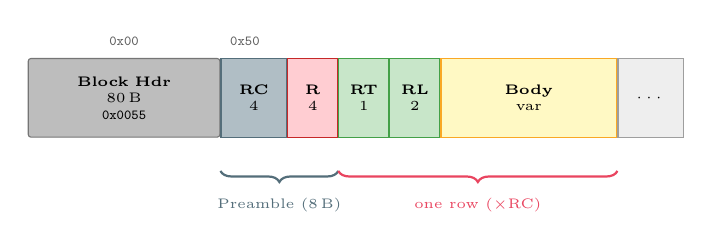
\begin{tikzpicture}[fld/.style={draw, minimum height=1.0cm, align=center, font=\tiny},lbl/.style={font=\tiny\ttfamily, color=muted}]
\node[fld, text width=2.2cm, fill=hdrBox, draw=hdrBoxB, rounded corners=1pt] (hdr) at (0,0) {\textbf{Block Hdr}\\80\,B\\\tiny\texttt{0x0055}};
\node[fld, text width=0.6cm, fill=fldPreamble, draw=fldPreambleB, right=0pt of hdr] (rc) {\textbf{RC}\\4};
\node[fld, text width=0.4cm, fill=colReserved, draw=colReservedB, right=0pt of rc] (r) {\textbf{R}\\4};
\node[fld, text width=0.4cm, fill=fldData, draw=fldDataB, right=0pt of r] (rt) {\textbf{RT}\\1};
\node[fld, text width=0.4cm, fill=fldData, draw=fldDataB, right=0pt of rt] (rl) {\textbf{RL}\\2};
\node[fld, text width=2.0cm, fill=fldVar, draw=fldVarB, right=0pt of rl] (body) {\textbf{Body}\\var};
\node[fld, text width=0.6cm, fill=fldMore, draw=fldMoreB, right=0pt of body] (more) {$\cdots$};
\node[lbl, above=1pt of hdr.north] {\hex{00}};
\node[lbl, above=1pt of rc.north west, anchor=south west] {\hex{50}};
\draw[decorate, decoration={brace, amplitude=4pt, mirror, raise=12pt}, thick, color=fldPreambleB] (rc.south west)--(r.south east) node[midway, below=18pt, font=\tiny\color{fldPreambleB}] {Preamble (8\,B)};
\draw[decorate, decoration={brace, amplitude=4pt, mirror, raise=12pt}, thick, color=accent] (rt.south west)--(body.south east) node[midway, below=18pt, font=\tiny\color{accent}] {one row ($\times$RC)};
\end{tikzpicture}}\caption{Connectivity Table (\hex{0055}). Abbreviations per Table~\ref{tab:block:ct} and Table~\ref{tab:block:ct-rows}.}\label{fig:connectivity-payload}\end{figure}



\subsection{Redaction and Data Minimization}\label{sec:redaction}
Investigation-mode fields such as \field{AcqUser}, \field{Hostname}, \field{Domain}, and \field{CaseRef} may contain personally identifiable information or data subject to disclosure restrictions. This section provides guidance for producers that must balance forensic completeness with privacy requirements.

\begin{itemize}[leftmargin=1.5em, itemsep=2pt]
\item Producers \MAY{} emit zero-length strings (Len=0) for \field{AcqUser}, \field{Domain}, and \field{CaseRef} when organizational policy requires data minimization. A conformant consumer \MUST{} handle zero-length optional strings gracefully.
\item When any field has been intentionally stripped or pseudonymized, producers \MUST{} set the \field{Redacted} flag (bit~3) in the file header. This distinguishes intentional redaction from fields that were merely unavailable at acquisition time: a zero-length string with \field{Redacted}=0 means ``not captured''; the same string with \field{Redacted}=1 means ``captured but removed.''
\item When sharing MSL files for research or cross-organizational analysis, producers \SHOULD{} strip or pseudonymize personally identifiable fields prior to distribution and set the \field{Redacted} flag.
\item \field{Hostname} and \field{OSDetail} carry forensic value that may be essential for investigation continuity. Redaction of these fields \SHOULD{} be documented in the case log.
\end{itemize}

%% ======================================================================
\section{Three-State Virtual Address Map}\label{sec:threestate}
%% ======================================================================
Each page within a Memory Region is classified into one of three states, encoded as 2~bits in the \field{PageStateMap}. This three-state model enforces \emph{epistemic honesty}: rather than silently omitting pages that could not be read, the format distinguishes successful capture from read failures and TOCTOU (Time-of-check to time-of-use)~races (pages that were mapped when the region was enumerated but absent when actually read). Table~\ref{tab:pagestates} defines the states; Figure~\ref{fig:pagestatemap} shows an example map.

\begin{table}[H]\centering\caption{Page states.}\label{tab:pagestates}\small
\begin{tabular}{M l p{5cm} l}\toprule\textbf{Bits}&\textbf{State}&\textbf{Meaning}&\textbf{PageData}\\\midrule
00 & Captured & Read OK; stored. & PageSize bytes \\
01 & Failed & Mapped but unreadable. & 0 \\
10 & Unmapped & TOCTOU: absent at read time. & 0 \\
11 & \textit{Reserved} & Treat as Failed. & 0 \\\bottomrule
\end{tabular}\end{table}

\begin{figure}[H]\centering
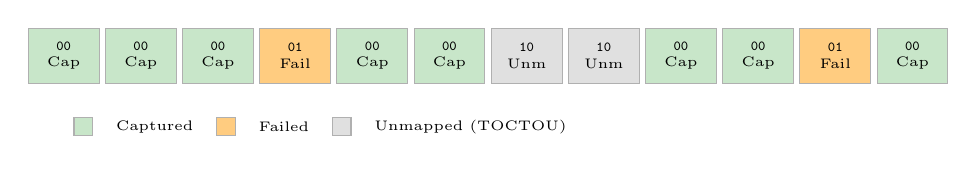
\begin{tikzpicture}[page/.style={draw=muted!50, minimum width=0.9cm, minimum height=0.7cm, align=center, font=\tiny}]
\foreach \i/\bits/\state/\col in {0/00/Cap/psCaptured,1/00/Cap/psCaptured,2/00/Cap/psCaptured,3/01/Fail/psFailed,4/00/Cap/psCaptured,5/00/Cap/psCaptured,6/10/Unm/psUnmapped,7/10/Unm/psUnmapped,8/00/Cap/psCaptured,9/00/Cap/psCaptured,10/01/Fail/psFailed,11/00/Cap/psCaptured}
{\node[page, fill=\col] at (\i*0.98,0) {\texttt{\bits}\\\state};}
\matrix[anchor=west] at (0,-0.9) [column sep=5pt, font=\tiny] {
\node[fill=psCaptured, draw=muted!50, minimum size=5pt] {}; & \node{Captured}; &
\node[fill=psFailed, draw=muted!50, minimum size=5pt] {}; & \node{Failed}; &
\node[fill=psUnmapped, draw=muted!50, minimum size=5pt] {}; & \node{Unmapped (TOCTOU)}; \\};
\end{tikzpicture}\caption{Example PageStateMap for a 12-page region.}\label{fig:pagestatemap}\end{figure}

%% ======================================================================
\section{Block Cross-Referencing}\label{sec:crossref}
%% ======================================================================
\textbf{Layer~1: \field{ParentUUID}.} Header-level hierarchy. Module Entry $\to$ Module List; system tables $\to$ System Context.

\textbf{Layer~2: Payload-embedded UUIDs.} Key Hint \field{RegionUUID} $\to$ Memory Region.

\begin{figure}[H]\centering
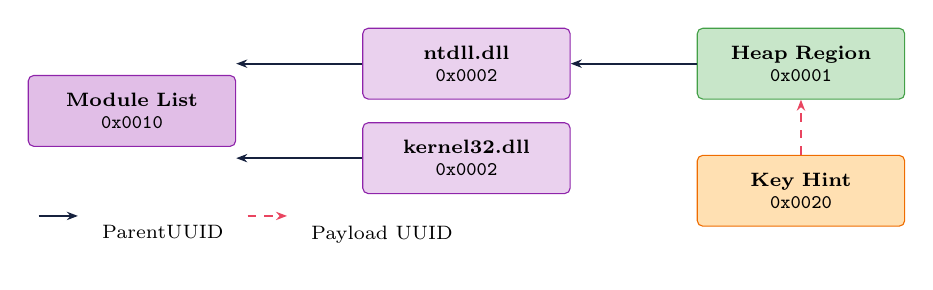
\begin{tikzpicture}[block/.style={draw, rounded corners=2pt, minimum height=0.9cm, align=center, font=\scriptsize, text width=2.4cm},parrow/.style={-{Stealth[length=4pt]}, thick, color=navy},earrow/.style={-{Stealth[length=4pt]}, thick, color=accent, dashed}]
\node[block, fill=btModule, draw=btModuleB] (mli) at (0,0) {\textbf{Module List}\\\hex{0010}};
\node[block, fill=btModule!70, draw=btModuleB, right=1.6cm of mli, yshift=0.6cm] (ntdll) {\textbf{ntdll.dll}\\\hex{0002}};
\node[block, fill=btModule!70, draw=btModuleB, right=1.6cm of mli, yshift=-0.6cm] (kern) {\textbf{kernel32.dll}\\\hex{0002}};
\node[block, fill=btMemRegion, draw=btMemRegionB, right=1.6cm of ntdll] (heap) {\textbf{Heap Region}\\\hex{0001}};
\node[block, fill=btKeyHint, draw=btKeyHintB, below=0.7cm of heap] (kh) {\textbf{Key Hint}\\\hex{0020}};
\draw[parrow] (ntdll.west)--(mli.east|-ntdll.west); \draw[parrow] (kern.west)--(mli.east|-kern.west);
\draw[parrow] (heap.west)--(ntdll.east); \draw[earrow] (kh.north)--(heap.south);
\matrix[below=0.7cm of mli.south west, anchor=north west, column sep=5pt, font=\scriptsize] {
\draw[parrow](0,0)--(0.5,0); & \node{ParentUUID}; & \draw[earrow](0,0)--(0.5,0); & \node{Payload UUID}; \\};
\end{tikzpicture}\caption{Block cross-referencing.}\label{fig:crossref}\end{figure}

\noindent\textbf{Dangling references.} Consumers encountering a \field{ParentUUID} or payload-embedded UUID that does not match any block in the file \SHOULD{} log the dangling reference and continue parsing. The block with the unresolvable reference \SHOULD{} be treated as an orphan but \MUSTNOT{} be discarded, as the referenced block may have been lost to corruption rather than being absent by design.
%% ======================================================================
\section{Capability Bitmap}\label{sec:capbitmap}
%% ======================================================================
The 64-bit \field{CapBitmap} in the file header advertises which categories of data the file contains. Consumers can inspect the bitmap before parsing any blocks to determine whether the information they need (e.g., module metadata, crypto key hints, system-wide tables) was captured. Each bit corresponds to one or more block types as shown in Table~\ref{tab:capbitmap}. Producers \MUST{} set bits accurately; consumers \SHOULD{} use the bitmap to report missing data categories rather than silently producing incomplete results.

\begin{table}[H]\centering\caption{Capability bits (64-bit \field{CapBitmap}).}\label{tab:capbitmap}\small
\begin{tabular}{l l p{6.5cm}}\toprule\textbf{Bit}&\textbf{Name}&\textbf{Description}\\\midrule
0 & MemoryRegions & \hex{0001}. \\ 1 & ModuleList & \hex{0010}/\hex{0002}. \\
2 & ThreadContexts & \hex{0011}. \\ 3 & FileDescriptors & \hex{0012}. \\
4 & NetworkState & \hex{0013}. \\ 5 & EnvironmentVars & \hex{0014}. \\
6 & SharedMemory & IPC identifiers. \\ 7 & SecurityContext & \hex{0015}. \\
8 & ProcessIdentity & \hex{0040}. \\ 9 & RelatedDumps & \hex{0041}. \\
10 & CryptoHints & \hex{0020}. \\
11 & SystemContext & \hex{0050}. \MUST{} be set when \field{Investigation} set. \\
12 & SystemProcessTable & \hex{0051}. \\ 13 & SystemNetworkTable & \hex{0052}. \\
14 & SystemHandleTable & \hex{0053}. \\ 15--63 & Reserved & Zero. \\\bottomrule
\end{tabular}\end{table}

%% ======================================================================
\newpage
\section{Encryption}\label{sec:encryption}
%% ======================================================================

\subsection{Scope}
When the \field{Encrypted} flag (bit~2) is set, the entire block stream is protected by AEAD (Authenticated Encryption with Associated Data). The file header remains in cleartext for format identification. All block data---including block types, UUIDs, timestamps, module paths, and memory content---is encrypted.

Full-container encryption is chosen over per-block encryption to prevent metadata leakage: per-block schemes would expose block types, block counts, block sizes, and timing patterns, all of which can reveal forensically sensitive information (e.g., which libraries are loaded, how many memory regions exist) without the decryption key.

\subsection{Encrypted File Layout}\label{sec:enclayout}

\begin{figure}[H]\centering
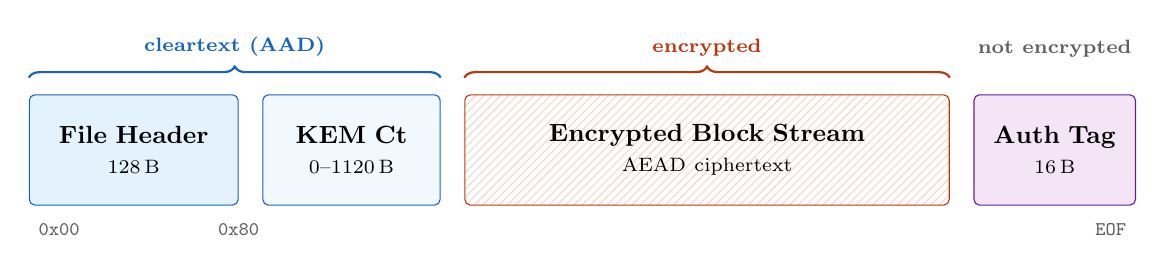
\begin{tikzpicture}[region/.style={draw, minimum height=1.4cm, align=center, font=\small, inner sep=5pt},lbl/.style={font=\scriptsize\ttfamily, color=muted},zonelbl/.style={font=\scriptsize\bfseries}]
\node[region, text width=2.3cm, fill=encClear, draw=encClearB, rounded corners=2pt] (hdr) at (0,0) {\textbf{File Header}\\\scriptsize 128\,B};
\node[region, text width=1.9cm, fill=encClear!50, draw=encClearB, rounded corners=2pt, right=0.3cm of hdr] (kem) {\textbf{KEM Ct}\\\scriptsize 0--1120\,B};
\node[region, text width=5.8cm, fill=encCipher, draw=encCipherB, rounded corners=2pt, right=0.3cm of kem, pattern=north east lines, pattern color=encCipherB!20] (cipher) {\textbf{Encrypted Block Stream}\\\scriptsize AEAD ciphertext};
\node[region, text width=1.7cm, fill=encTag, draw=encTagB, rounded corners=2pt, right=0.3cm of cipher] (tag) {\textbf{Auth Tag}\\\scriptsize 16\,B};
\node[lbl, below=3pt of hdr.south west, anchor=north west] {0x00}; \node[lbl, below=3pt of hdr.south east, anchor=north] {0x80}; \node[lbl, below=3pt of tag.south east, anchor=north east] {EOF};
\draw[decorate, decoration={brace, amplitude=4pt, raise=6pt}, thick, color=encClearB] (hdr.north west)--(kem.north east) node[midway, above=10pt, zonelbl, color=encClearB] {cleartext (AAD)};
\draw[decorate, decoration={brace, amplitude=4pt, raise=6pt}, thick, color=encCipherB] (cipher.north west)--(cipher.north east) node[midway, above=10pt, zonelbl, color=encCipherB] {encrypted};
\node[zonelbl, color=muted, above=10pt of tag.north] {not encrypted};
\end{tikzpicture}\caption{Encrypted file layout. The AEAD encrypts the block stream; the tag is an output, not itself encrypted.}\label{fig:enc-layout}\end{figure}

\begin{enumerate}[leftmargin=1.8em, itemsep=2pt]
\item \textbf{File header (128\,B, cleartext):} Authenticated as Associated Data (AAD) to the AEAD, along with any KEM ciphertext. Tampering causes decryption failure.
\item \textbf{KEM ciphertext (0 or variable, cleartext):} Present when \field{KeyEncap}$\neq$\hex{00}. Size is \field{KEMCtLen}. Also in AAD.
\item \textbf{Encrypted block stream:} AEAD ciphertext of Block~0 through EoC. The only encrypted region.
\item \textbf{AEAD authentication tag (16\,B, not encrypted):} Output of the AEAD. Required for decryption. Requires the symmetric key.
\end{enumerate}

\noindent\textbf{Chain-of-custody without the key.} Producers \SHOULD{} record an external hash of the complete file at acquisition time (\blake{} or SHA-256, offset~0 to EOF). This digest \SHOULD{} be stored in the case evidence log, not in the file.

\subsection{Cipher Suites}
\begin{table}[H]\centering\caption{AEAD cipher suites.}\label{tab:ciphers}\small
\begin{tabular}{M l l l p{3.5cm}}\toprule\textbf{Code}&\textbf{Suite}&\textbf{Nonce}&\textbf{Tag}&\textbf{Notes}\\\midrule
0x01 & AES-256-GCM & 12\,B & 16\,B & Default. Fast with AES-NI. \\
0x02 & XChaCha20-Poly1305 & 24\,B & 16\,B & Safe random nonce. \\\bottomrule
\end{tabular}\end{table}

\noindent Both ciphers provide 256-bit keys. AES-256 and ChaCha20 are post-quantum safe at the symmetric level (Grover reduces effective key strength by half: AES-256 $\to$ 128-bit equivalent). The post-quantum vulnerability lies in key \emph{encapsulation}, addressed below.

\subsection{Key Encapsulation}\label{sec:kem}
The \field{KeyEncap} field specifies how the content encryption key (CEK) was protected. After KEM decapsulation, the shared secret is passed through HKDF-\blake{} (salt=\field{DumpUUID}, info=\texttt{"MSL-CEK-v1"}) to derive the 256-bit CEK.

\begin{table}[H]\centering\caption{Key encapsulation mechanisms.}\label{tab:kem}\small
\begin{tabular}{M l l p{4.5cm}}\toprule\textbf{Code}&\textbf{Mechanism}&\textbf{Ct Size}&\textbf{Notes}\\\midrule
0x00 & None & 0 & Raw key (passphrase or external). \\
0x01 & X25519 & 32\,B & Classical ECDH. \\
0x02 & ML-KEM-768 & 1088\,B & FIPS~203~\cite{mlkem}. NIST PQ standard. \\
0x03 & ML-KEM-1024 & 1568\,B & FIPS~203. Higher margin. \\
0x04 & X25519+ML-KEM-768 & 1120\,B & Hybrid. \textbf{Recommended.} \\
0x05--0xFE & \textit{Reserved} & --- & \\
0xFF & Other & var & Non-standard. \\\bottomrule
\end{tabular}\end{table}

\begin{notebox}[title={Operational model: symmetric key vs.\ KEM}]
The symmetric cipher always encrypts the data. \field{KeyEncap} determines how the CEK reaches the intended recipient:
\begin{itemize}[leftmargin=1.5em, itemsep=2pt]
\item \textbf{\field{KeyEncap}=\hex{00} (passphrase/raw key):} The responder provides a passphrase or externally managed key. Suitable for single-operator scenarios.
\item \textbf{\field{KeyEncap}$\neq$\hex{00} (KEM):} The acquirer encrypts to the organization's public key. The responder need not know any secret. The private key is held by the analysis team or in an HSM. This provides separation of duties: the responder who captures evidence cannot decrypt it.
\item \textbf{Passphrase + KEM (dual control):} Both the responder's passphrase and the organization's private key are required, preventing either party from accessing evidence alone.
\end{itemize}
\noindent The post-quantum options protect against ``harvest now, decrypt later'' attacks.
\end{notebox}

\noindent\textbf{Hybrid X25519 + ML-KEM-768.} The recommended hybrid scheme (\hex{04}) concatenates shared secrets from X25519 and ML-KEM-768 before KDF, ensuring the file remains secure as long as \emph{either} assumption holds. This concatenate-then-KDF construction follows the approach analyzed by Bindel et al.~\cite{bindel2019} and adopted by TLS~1.3 hybrid key exchange~\cite{ietfhybrid}. The hybrid mode is the \textbf{recommended} setting for Investigation mode captures.

\subsection{Key Derivation}
\begin{description}[style=nextline, leftmargin=2em, itemsep=3pt]
\item[\hex{00} --- None] 256-bit CEK provided externally. KDF fields are zero.
\item[\hex{01} --- Argon2id] Passphrase-derived. Minimum: time=3, memory=65536\,KiB, lanes=4.
\end{description}

\noindent Because \field{KDFSalt} is generated uniquely per file (16 random bytes), the same passphrase produces a different CEK for each capture, eliminating nonce-reuse risk even when nonces are generated independently across files.

\subsection{Interaction with the Integrity Chain}\label{sec:enc-integrity}
When \field{Encrypted} is set:
\begin{itemize}[leftmargin=1.5em, itemsep=2pt]
\item \field{PrevHash}: \MUST{} be zero. AEAD authenticates atomically.
\item EoC \field{FileHash}: \SHOULD{} be computed over plaintext (enables post-decryption verification).
\item AAD: File header (128\,B) + any KEM ciphertext.
\end{itemize}

\subsection{Streaming Encryption}
Producers \SHOULD{} encrypt incrementally: (1)~init AEAD with key, nonce, AAD; (2)~for each block, serialize, encrypt, write; (3)~after EoC, finalize AEAD, append 16-byte tag. A parallel \blake{} hasher computes plaintext FileHash before encryption. $O(1)$ memory.

%% ======================================================================
\newpage
\section{Raw Dump Import}\label{sec:import}
%% ======================================================================
An MSL file may be created by importing a pre-existing raw memory dump (ELF core, Windows Minidump, ProcDump output, or plain byte stream) rather than by live acquisition. The Import Provenance block (\hex{0030}) records the origin of the imported data: the source format, the tool that performed the conversion, the original file size, and an optional free-text note. When \field{Imported} (bit~0) is set in \field{Flags}, this block \MUST{} appear as Block~0.

\begin{table}[H]\centering\caption{Import Provenance payload.}\label{tab:importprov}\small
\begin{tabular}{M M l p{5cm}}\toprule\textbf{Off}&\textbf{Size}&\textbf{Field}&\textbf{Description}\\\midrule
+0x00 & 2 & \field{SourceFormat} & Table~\ref{tab:srcfmt}. \\
+0x02 & 2 & \field{Reserved} & Zero. \\
+0x04 & 4 & \field{ToolNameLen} & Incl.\ null. \\
+0x08 & 8 & \field{ImportTime} & ns since epoch. \\
+0x10 & 8 & \field{OrigFileSize} & 0 if unknown. \\
+0x18 & 4 & \field{NoteLen} & 0 if none. \\
+0x1C & 4 & \field{Reserved2} & Zero. \\
+0x20 & var & \field{ToolName} & UTF-8, pad8. \\
$+t$ & var & \field{Note} & UTF-8, pad8. \\\bottomrule
\end{tabular}\end{table}

\begin{table}[H]\centering\caption{Source format codes.}\label{tab:srcfmt}\small
\begin{tabular}{M l}\toprule\textbf{Code}&\textbf{Format}\\\midrule
0x0000 & Unknown \\ 0x0001 & Raw byte stream \\ 0x0002 & ELF core dump \\ 0x0003 & Windows Minidump \\ 0x0004 & macOS core dump \\ 0x0005 & ProcDump \\ 0xFFFF & Other \\\bottomrule
\end{tabular}\end{table}

\noindent\textbf{Procedure:} (1) Set \field{Flags} bit~0. (2) Block~0: Import Provenance. (3) Regions from source. (4) Modules if available. (5) Hash chain and EoC.

%% ======================================================================
\section{Parsing Walkthrough}\label{sec:parsing}
%% ======================================================================
\begin{description}[style=nextline, leftmargin=2em, itemsep=4pt]
\item[Step 1:] Read 9 bytes. Verify magic. \field{Endianness} \MUST{} be \hex{01}. Read \field{HeaderSize}.
\item[Step 2:] If \field{Encrypted}: read extension (\hex{40}--\hex{7F}). If \field{KEMCtLen}$>$0, read KEM ciphertext. Obtain key. Decrypt. Continue with plaintext.
\item[Step 3:] Read blocks at \field{HeaderSize} (+\field{KEMCtLen} if encrypted). Verify \field{BlockLength}$\geq$80. Parse or skip via \field{BlockLength}. If \field{BlockCount}$>$0, verify parsed count matches.
\item[Step 4:] If unencrypted: verify \blake{} chain. If encrypted: verify AEAD tag.
\item[Step 5:] Verify EoC \field{FileHash} if present.
\item[Step 6:] \field{Investigation}? Expect Block~2 = System Context.
\item[Step 7:] \field{Imported}? Read Import Provenance.
\end{description}

%% ======================================================================
\newpage
\section{Worked Example}\label{sec:example}
%% ======================================================================
Module Entry block for \texttt{ntdll.dll} v\texttt{10.0.22621.1} at \hex{7FFDD4D00000}. Path=30B (pad8=32). Version=13B (pad8=16). Payload=496B. Block=576 (\hex{0240}).

\begin{table}[H]\centering\caption{ntdll.dll Module Entry.}\label{tab:example}\small
\begin{tabular}{M l l p{3.5cm}}\toprule\textbf{Off}&\textbf{Field}&\textbf{Hex}&\textbf{Value}\\\midrule
\multicolumn{4}{l}{\textit{--- Header (80B) ---}} \\
0x00 & Magic & \texttt{4D 53 4C 43} & MSLC \\
0x04 & BlockType & \texttt{02 00} & Module Entry \\
0x08 & BlockLength & \texttt{40 02 00 00} & 576 \\
0x0C & PayloadVersion & \texttt{01 00} & 1 \\
0x10 & BlockUUID & (16B) & UUIDv4 \\
0x20 & ParentUUID & (16B) & Module List UUID \\
0x30 & PrevHash & (32B) & \blake{} of prev \\
\midrule\multicolumn{4}{l}{\textit{--- Payload (496B) ---}} \\
0x50 & BaseAddr & \texttt{00 00 D0 D4 FD 7F 00 00} & \hex{7FFDD4D00000} \\
0x58 & ModuleSize & \texttt{00 00 20 00 00 00 00 00} & 2\,MiB \\
0x60 & PathLen & \texttt{1E 00} & 30 \\
0x62 & VersionLen & \texttt{0D 00} & 13 \\
0x68 & Path (32B) & \texttt{43 3A 5C 57\ldots} & ntdll.dll \\
0x88 & Version (16B) & \texttt{31 30 2E 30\ldots} & 10.0.22621.1 \\
0x98 & DiskHash (32B) & \ldots & \blake{} of binary \\
0xB8 & BlobLen & \texttt{80 01 00 00} & 384 \\
0xC0 & NativeBlob & (384B) & LDR\_DATA\_TABLE\_ENTRY \\\bottomrule
\end{tabular}\end{table}

%% ======================================================================
\newpage
\section{Conformance}\label{sec:conformance}
%% ======================================================================
\subsection{Producer}
A conformant producer \MUST: (1) write valid header with \field{Magic}, \field{Endianness}=\hex{01}, \field{HeaderSize}, \field{Version}; (2) generate UUIDv4 in RFC~9562 binary layout; (3) compute \blake{} \field{PrevHash} (zero when encrypted); (4) set reserved fields to zero; (5) pad8 all variable fields; (6) never modify written blocks; (7) set \field{CapBitmap} accurately; (8) if importing: set \field{Flags} bit~0, emit Import Provenance as Block~0; (9) set \field{PayloadVersion} to~1; (10) set \field{CompAlgo} bits to 00 when uncompressed; (11) split regions exceeding $2^{32}{-}81$ bytes; (12) write 32 zero bytes for unavailable \field{DiskHash}; (13) reject \field{PageSizeLog2} outside $[10,40]$; (14) emit well-formed UTF-8 per RFC~3629 for all string fields; (15) convert port numbers from network byte order to little-endian before writing; (16) set \field{BlockCount} to the total number of blocks or zero if unknown.

A conformant acquirer \MUST{} emit Process Identity as Block~0 and Module List Index as Block~1.

\noindent\textbf{Investigation:} (17) emit System Context as Block~2; (18) set \field{CapBitmap} bit~11; (19) set \field{TableBitmap}; (20) set \field{Redacted} flag (bit~3) when any field has been intentionally stripped or pseudonymized.

\noindent\textbf{Encryption:} (21) \field{HeaderSize}=128; (22) valid encryption extension; (23) AEAD with header (+KEM ct) as AAD; (24) append 16-byte tag; (25) zero all \field{PrevHash}; (26) \field{Nonce} from CSPRNG; (27) KEM ciphertext after header when \field{KeyEncap}$\neq$\hex{00}.

\noindent\textbf{Compression:} (28) when \field{Compressed} is set, write 8-byte \field{UncompressedSize} before compressed data; (29) set \field{BlockLength} to on-disk size.

\noindent\textbf{Block types:} (30) \MUSTNOT{} emit block types whose payload format is not yet specified in this document.
\noindent\textbf{Hash algorithm:} (31) set \field{HashAlgo} to a registered code from Table~\ref{tab:hashalgos}; the default (\hex{00}, BLAKE3) \SHOULD{} be used unless FIPS compliance, organizational policy, or platform performance measurements indicate otherwise; (32) use the selected algorithm exclusively for all \field{PrevHash}, \field{FileHash}, and \field{DiskHash} computations within the file; \MUSTNOT{} mix algorithms within a single file.

\noindent A producer \SHOULD{} emit an EoC block. \field{FileHash} \SHOULD{} be computed over plaintext even when encrypted. When encrypted, the producer \SHOULD{} record an external file hash for chain-of-custody.

\subsection{Consumer}
A conformant consumer \MUST: (1) reject invalid magic or \field{Endianness}$\neq$\hex{01}; (2) use \field{HeaderSize} to locate blocks; (3) skip unknown types via \field{BlockLength}; (4) reject $\field{BlockLength} < 80$; (5) detect end-of-blocks; (6) ignore reserved fields; (7) reject type \hex{0000}; (8) skip unrecognized \field{PayloadVersion} for known block types with a logged warning indicating which block types were affected; (9) treat all-zero \field{DiskHash} as unavailable; (10) reject \field{PageSizeLog2} outside $[10,40]$; (11) use explicit length fields to determine string extent, not NUL-scanning beyond the declared length; (12) preserve raw bytes for malformed UTF-8 fields and not reject the entire block; (13) if \field{BlockCount}$>$0, verify parsed count matches; (14) treat bytes after a verified EoC as trailing non-MSL data.

\noindent\textbf{Encryption:} (15) verify \field{HeaderSize}=128; read KEM ct; decrypt via AEAD with AAD; reject on failure; (16) skip \field{PrevHash} verification.

\noindent\textbf{Investigation:} (17) expect Block~2 = System Context; check \field{TableBitmap}; (18) when \field{Redacted} is set, interpret zero-length optional strings as intentionally redacted rather than absent.

\noindent\textbf{Compression:} (19) read 8-byte \field{UncompressedSize} before inflating; (20) reject if decompressed size does not match \field{UncompressedSize}.

\noindent\textbf{Cross-references:} (21) log and continue on dangling \field{ParentUUID} or payload-embedded UUID references; treat the affected block as an orphan but \MUSTNOT{} discard it.
\noindent\textbf{Hash algorithm:} (22) \MUST{} implement at minimum \field{HashAlgo}=\hex{00} (BLAKE3) and \field{HashAlgo}=\hex{01} (SHA-256); \MAY{} implement \hex{02} (SHA-512/256) and other registered codes; \MUST{} reject files whose \field{HashAlgo} the consumer does not implement, emitting a diagnostic indicating the unsupported algorithm code.

\noindent A consumer \SHOULD: verify \blake{} chain when unencrypted; verify EoC \field{FileHash} after decryption.

\clearpage
\begin{thebibliography}{9}
\bibitem{rfc2119} S.~Bradner, ``Key words for use in RFCs to Indicate Requirement Levels,'' RFC~2119, 1997.
\bibitem{rfc9562} K.~Davis, B.~Peabody, P.~Leach, ``Universally Unique IDentifiers (UUIDs),'' RFC~9562, 2024.
\bibitem{rfc3629} F.~Yergeau, ``UTF-8, a transformation format of ISO 10646,'' RFC~3629, 2003.
\bibitem{blake3} J.~O'Connor et al., ``BLAKE3: One function, fast everywhere,'' 2020. \url{https://github.com/BLAKE3-team/BLAKE3-specs/blob/master/blake3.pdf}
\bibitem{fips180} NIST, ``Secure Hash Standard (SHS),'' FIPS~180-4, 2015. \url{https://doi.org/10.6028/NIST.FIPS.180-4}
\bibitem{elf} TIS Committee, ``ELF Specification,'' v1.2, 1995.
\bibitem{mlkem} NIST, ``Module-Lattice-Based Key-Encapsulation Mechanism Standard,'' FIPS~203, 2024. \url{https://doi.org/10.6028/NIST.FIPS.203}
\bibitem{bindel2019} N.~Bindel, J.~Brendel, M.~Fischlin, B.~Goncalves, D.~Stebila, ``Hybrid Key Encapsulation Mechanisms and Authenticated Key Exchange,'' in \emph{Post-Quantum Cryptography (PQCrypto)}, Springer, 2019.
\bibitem{ietfhybrid} D.~Stebila, S.~Fluhrer, S.~Gueron, ``Hybrid key exchange in TLS 1.3,'' Internet-Draft draft-ietf-tls-hybrid-design, IETF, 2024.
\end{thebibliography}

\end{document}